% Options for packages loaded elsewhere
\PassOptionsToPackage{unicode}{hyperref}
\PassOptionsToPackage{hyphens}{url}
\documentclass[
]{article}
\usepackage{xcolor}
\usepackage{amsmath,amssymb}
\setcounter{secnumdepth}{5}
\usepackage{iftex}
\ifPDFTeX
  \usepackage[T1]{fontenc}
  \usepackage[utf8]{inputenc}
  \usepackage{textcomp} % provide euro and other symbols
\else % if luatex or xetex
  \usepackage{unicode-math} % this also loads fontspec
  \defaultfontfeatures{Scale=MatchLowercase}
  \defaultfontfeatures[\rmfamily]{Ligatures=TeX,Scale=1}
\fi
% \usepackage{lmodern}
\ifPDFTeX\else
  % xetex/luatex font selection
\fi
% Use upquote if available, for straight quotes in verbatim environments
\IfFileExists{upquote.sty}{\usepackage{upquote}}{}
\IfFileExists{microtype.sty}{% use microtype if available
  \usepackage[]{microtype}
  \UseMicrotypeSet[protrusion]{basicmath} % disable protrusion for tt fonts
}{}
\makeatletter
\@ifundefined{KOMAClassName}{% if non-KOMA class
  \IfFileExists{parskip.sty}{%
    \usepackage{parskip}
  }{% else
    \setlength{\parindent}{0pt}
    \setlength{\parskip}{6pt plus 2pt minus 1pt}}
}{% if KOMA class
  \KOMAoptions{parskip=half}}
\makeatother
\usepackage{color}
\usepackage{fancyvrb}
\newcommand{\VerbBar}{|}
\newcommand{\VERB}{\Verb[commandchars=\\\{\}]}
\DefineVerbatimEnvironment{Highlighting}{Verbatim}{commandchars=\\\{\}}
% Add ',fontsize=\small' for more characters per line
\newenvironment{Shaded}{}{}
\newcommand{\AlertTok}[1]{\textcolor[rgb]{1.00,0.00,0.00}{\textbf{#1}}}
\newcommand{\AnnotationTok}[1]{\textcolor[rgb]{0.38,0.63,0.69}{\textbf{\textit{#1}}}}
\newcommand{\AttributeTok}[1]{\textcolor[rgb]{0.49,0.56,0.16}{#1}}
\newcommand{\BaseNTok}[1]{\textcolor[rgb]{0.25,0.63,0.44}{#1}}
\newcommand{\BuiltInTok}[1]{\textcolor[rgb]{0.00,0.50,0.00}{#1}}
\newcommand{\CharTok}[1]{\textcolor[rgb]{0.25,0.44,0.63}{#1}}
\newcommand{\CommentTok}[1]{\textcolor[rgb]{0.38,0.63,0.69}{\textit{#1}}}
\newcommand{\CommentVarTok}[1]{\textcolor[rgb]{0.38,0.63,0.69}{\textbf{\textit{#1}}}}
\newcommand{\ConstantTok}[1]{\textcolor[rgb]{0.53,0.00,0.00}{#1}}
\newcommand{\ControlFlowTok}[1]{\textcolor[rgb]{0.00,0.44,0.13}{\textbf{#1}}}
\newcommand{\DataTypeTok}[1]{\textcolor[rgb]{0.56,0.13,0.00}{#1}}
\newcommand{\DecValTok}[1]{\textcolor[rgb]{0.25,0.63,0.44}{#1}}
\newcommand{\DocumentationTok}[1]{\textcolor[rgb]{0.73,0.13,0.13}{\textit{#1}}}
\newcommand{\ErrorTok}[1]{\textcolor[rgb]{1.00,0.00,0.00}{\textbf{#1}}}
\newcommand{\ExtensionTok}[1]{#1}
\newcommand{\FloatTok}[1]{\textcolor[rgb]{0.25,0.63,0.44}{#1}}
\newcommand{\FunctionTok}[1]{\textcolor[rgb]{0.02,0.16,0.49}{#1}}
\newcommand{\ImportTok}[1]{\textcolor[rgb]{0.00,0.50,0.00}{\textbf{#1}}}
\newcommand{\InformationTok}[1]{\textcolor[rgb]{0.38,0.63,0.69}{\textbf{\textit{#1}}}}
\newcommand{\KeywordTok}[1]{\textcolor[rgb]{0.00,0.44,0.13}{\textbf{#1}}}
\newcommand{\NormalTok}[1]{#1}
\newcommand{\OperatorTok}[1]{\textcolor[rgb]{0.40,0.40,0.40}{#1}}
\newcommand{\OtherTok}[1]{\textcolor[rgb]{0.00,0.44,0.13}{#1}}
\newcommand{\PreprocessorTok}[1]{\textcolor[rgb]{0.74,0.48,0.00}{#1}}
\newcommand{\RegionMarkerTok}[1]{#1}
\newcommand{\SpecialCharTok}[1]{\textcolor[rgb]{0.25,0.44,0.63}{#1}}
\newcommand{\SpecialStringTok}[1]{\textcolor[rgb]{0.73,0.40,0.53}{#1}}
\newcommand{\StringTok}[1]{\textcolor[rgb]{0.25,0.44,0.63}{#1}}
\newcommand{\VariableTok}[1]{\textcolor[rgb]{0.10,0.09,0.49}{#1}}
\newcommand{\VerbatimStringTok}[1]{\textcolor[rgb]{0.25,0.44,0.63}{#1}}
\newcommand{\WarningTok}[1]{\textcolor[rgb]{0.38,0.63,0.69}{\textbf{\textit{#1}}}}
\usepackage{longtable,booktabs,array}
\newcounter{none} % for unnumbered tables
\usepackage{calc} % for calculating minipage widths
% Correct order of tables after \paragraph or \subparagraph
\usepackage{etoolbox}
\makeatletter
\patchcmd\longtable{\par}{\if@noskipsec\mbox{}\fi\par}{}{}
\makeatother
% Allow footnotes in longtable head/foot
\IfFileExists{footnotehyper.sty}{\usepackage{footnotehyper}}{\usepackage{footnote}}
\makesavenoteenv{longtable}
\usepackage{graphicx}
\makeatletter
\newsavebox\pandoc@box
\newcommand*\pandocbounded[1]{% scales image to fit in text height/width
  \sbox\pandoc@box{#1}%
  \Gscale@div\@tempa{\textheight}{\dimexpr\ht\pandoc@box+\dp\pandoc@box\relax}%
  \Gscale@div\@tempb{\linewidth}{\wd\pandoc@box}%
  \ifdim\@tempb\p@<\@tempa\p@\let\@tempa\@tempb\fi% select the smaller of both
  \ifdim\@tempa\p@<\p@\scalebox{\@tempa}{\usebox\pandoc@box}%
  \else\usebox{\pandoc@box}%
  \fi%
}
% Set default figure placement to htbp
\def\fps@figure{htbp}
\makeatother
\setlength{\emergencystretch}{3em} % prevent overfull lines
\providecommand{\tightlist}{%
  \setlength{\itemsep}{0pt}\setlength{\parskip}{0pt}}
\usepackage[]{natbib}
\bibliographystyle{plainnat}
\makeatletter
\@ifpackageloaded{subcaption}{}{\usepackage{subcaption}}
\@ifpackageloaded{caption}{}{\usepackage{caption}}
\captionsetup[subfigure]{margin=0.5em}
\AtBeginDocument{%
\renewcommand*\figurename{Figure}
\renewcommand*\tablename{Table}
}
\AtBeginDocument{%
\renewcommand*\listfigurename{List of Figures}
\renewcommand*\listtablename{List of Tables}
}
\newcounter{pandoccrossref@subfigures@footnote@counter}
\newenvironment{pandoccrossrefsubfigures}{%
\setcounter{pandoccrossref@subfigures@footnote@counter}{0}
\begin{figure}\centering%
\gdef\global@pandoccrossref@subfigures@footnotes{}%
\DeclareRobustCommand{\footnote}[1]{\footnotemark%
\stepcounter{pandoccrossref@subfigures@footnote@counter}%
\ifx\global@pandoccrossref@subfigures@footnotes\empty%
\gdef\global@pandoccrossref@subfigures@footnotes{{##1}}%
\else%
\g@addto@macro\global@pandoccrossref@subfigures@footnotes{, {##1}}%
\fi}}%
{\end{figure}%
\addtocounter{footnote}{-\value{pandoccrossref@subfigures@footnote@counter}}
\@for\f:=\global@pandoccrossref@subfigures@footnotes\do{\stepcounter{footnote}\footnotetext{\f}}%
\gdef\global@pandoccrossref@subfigures@footnotes{}}
\@ifpackageloaded{float}{}{\usepackage{float}}
\floatstyle{ruled}
\@ifundefined{c@chapter}{\newfloat{codelisting}{h}{lop}}{\newfloat{codelisting}{h}{lop}[chapter]}
\floatname{codelisting}{Listing}
\newcommand*\listoflistings{\listof{codelisting}{List of Listings}}
\makeatother
\usepackage{bookmark}
\IfFileExists{xurl.sty}{\usepackage{xurl}}{} % add URL line breaks if available
\urlstyle{same}
% fallback for those not using the hyperref driver hyperxmp:
\makeatletter
\@ifundefined{xmpquote}{\newcommand{\xmpquote}[1]{#1}}{}
\makeatother
\hypersetup{
  colorlinks=true,linkcolor=red,urlcolor=red,citecolor=red,anchorcolor=red,filecolor=red,
  pdfcreator={LaTeX via pandoc}}

\author{}
\date{}

\IfFileExists{seqsplit.sty}{\usepackage{seqsplit}}{\newcommand{\seqsplit}[1]{#1}}
\protected\def\breakseq#1{\seqsplit{#1}}
\protected\def\breaktt#1{\begingroup\ttfamily\seqsplit{#1}\endgroup}
\title{Reproducible Literature Synthesis with infrastructure/search and infrastructure/reference}
\author{Research Template Author\\\footnotesize{Research Template Institute}\\\footnotesize{\texttt{author@research-template.org}}\\\footnotesize{\href{https://orcid.org/0000-0000-0000-1234}{ORCID: 0000-0000-0000-1234}}}
\date{\today}

\usepackage{amsmath}
\usepackage{amssymb}
\usepackage{geometry}
\usepackage{graphicx}
\usepackage{booktabs}
\usepackage{longtable}
\usepackage{hyperref}
\usepackage{cleveref}
\usepackage{xcolor}
\usepackage{listings}
\geometry{margin=1in}
\hypersetup{colorlinks=true, linkcolor=blue, citecolor=teal, urlcolor=teal}

\begin{document}

\begin{titlepage}
\centering
\vspace*{2cm}
{\LARGE\bfseries Reproducible Literature Synthesis with infrastructure/search and infrastructure/reference\par}
\vspace{0.75em}
{\large A configurable pipeline from query → references.bib → LLM-driven reading report\par}
\vfill
\makeatletter
{\@author\par}
\vspace{1em}
{\@date\par}
\makeatother
\vfill
\end{titlepage}
\thispagestyle{empty}
\tableofcontents
\newpage


\section{Abstract}\label{sec:abstract}

This paper documents \breaktt{template\_search\_project}, the
literature-search exemplar shipped with the
\href{https://github.com/docxology/template}{Research Project Template}.
The project demonstrates \textbf{two configurable, reproducible
pipelines} sharing the same configuration file and the same
\breaktt{infrastructure/search/} + \breaktt{infrastructure/reference/}
modules. The standard pipeline
(\breaktt{scripts/run\_search\_pipeline.py}) handles a single
\texttt{SearchQuery} end-to-end. The deep-search pipeline
(\breaktt{scripts/run\_deep\_search.py}, see sec.~\ref{sec:deep_search})
fans out across a list of keywords (each capped at 100 papers per
keyword from \breaktt{deep\_search.max\_results\_per\_keyword} in
\breaktt{manuscript/config.yaml}), fully enriches every paper with its
abstract and PDF fulltext, and (optionally) uses the local LLM to write
a multi-section reading note for every paper. When a deep-search
aggregate exists, the latest run covered \textbf{3} keyword(s) with
\textbf{} unique paper(s) after cross-keyword deduplication. Both turn a
free-text topic into:

\begin{enumerate}
\def\labelenumi{\arabic{enumi}.}
\tightlist
\item
  a deduplicated, year-filtered set of papers drawn from arXiv,
  Crossref, optional local corpora, and (opt-in)
  \href{https://paperclip.gxl.ai/}{Paperclip};
\item
  a Pandoc-compatible \texttt{references.bib} byte-identical in style to
  the canonical exemplar in
  \href{../../template_code_project/manuscript/references.bib}{\breaktt{template\_code\_project}}
  (file \breaktt{manuscript/references.bib});
\item
  cached abstracts and (optionally) extracted PDF full text, written to
  disk under stable per-paper identifiers; and
\item
  an LLM-synthesised reading report assembled from per-paper analyses
  and a cross-corpus thematic synthesis, all produced by a local Ollama
  model with pinned seed and temperature.
\end{enumerate}

All discovery logic lives in \breaktt{infrastructure/search/literature/}
(\href{https://github.com/docxology/template/tree/main/infrastructure/search/literature}{source
on GitHub}); all export logic lives in
\breaktt{infrastructure/reference/citation/}
(\href{https://github.com/docxology/template/tree/main/infrastructure/reference/citation}{source
on GitHub}); LLM synthesis reuses the existing
\breaktt{infrastructure/llm/}
(\href{https://github.com/docxology/template/tree/main/infrastructure/llm}{source
on GitHub}) bridge. The project itself contains only thin orchestration,
manuscript prose, and a test suite --- perfectly mirroring the
\textbf{two-layer architecture} the template enforces.

The motivating concern is \emph{reproducibility}: a query at time
\(t_0\) should produce the same results at time \(t_1\) unless the cache
is explicitly invalidated. This is achieved by deterministic search
caching keyed on canonical query identity, on-disk caching of every
fetched abstract / PDF, and pinned LLM seeds. The same
\breaktt{manuscript/config.yaml} that drives the pipeline is also the
only configuration any reviewer needs.

\textbf{Run snapshot.} With the bundled \breaktt{manuscript/config.yaml},
the most recent pipeline execution evaluated the query
\emph{``reproducible research optimization''} against local, returned 6
deduplicated paper(s) (4 carrying a DOI, 6 carrying an abstract), and
recorded backend errors: none. Resolve \texttt{\{\{…\}\}} tokens by
running \breaktt{scripts/z\_generate\_manuscript\_variables.py} after
\breaktt{run\_search\_pipeline.py}; the script writes
\breaktt{output/data/manuscript\_variables.json} and resolved markdown
under \breaktt{output/manuscript/}, which the PDF-rendering stage prefers
when present.

\textbf{Keywords:} literature search, BibTeX automation, reproducible
research, local LLM synthesis, scientific infrastructure

\newpage

\section{Introduction}\label{sec:introduction}

Reproducible computational research demands that every claim be
traceable back to a stable artifact --- code, data, and citations alike
\citep{peng2011reproducible}. Manual literature curation is a well-known
bottleneck in such workflows: a graduate student writing a related-work
section may spend hours searching arXiv, Crossref, and Google Scholar;
copying citations into a \texttt{.bib} file by hand; and tracking which
papers they have actually read. Three failure modes recur:

\begin{enumerate}
\def\labelenumi{\arabic{enumi}.}
\tightlist
\item
  \textbf{Style drift} --- hand-edited \texttt{.bib} files accumulate
  formatting inconsistencies that hide real semantic conflicts in
  version-control diffs.
\item
  \textbf{Stale state} --- the bibliography, the reading list, and the
  manuscript prose drift apart as the project evolves; the citation key
  in the manuscript no longer matches the entry in \texttt{.bib}, or the
  entry no longer matches the actual paper.
\item
  \textbf{Lost context} --- abstracts and full text are read once during
  search, then discarded; six months later the same paper has to be
  re-skimmed to recall its contribution.
\end{enumerate}

\breaktt{template\_search\_project} exists to demonstrate one disciplined
solution. The pipeline outputs are summarised in
sec.~\ref{sec:methodology} (overview figure at the start of that
section):

\begin{itemize}
\tightlist
\item
  The discovery side
  (\href{../../../../infrastructure/search/}{\breaktt{infrastructure/search/}})
  provides multi-source paper search with failure-isolated aggregation,
  DOI/arXiv-aware deduplication, and deterministic JSON caching keyed on
  canonical query identity.
\item
  The export side
  (\href{../../../../infrastructure/reference/}{\breaktt{infrastructure/reference/}})
  provides BibTeX read/write/convert facilities byte-compatible with the
  existing exemplar \texttt{references.bib}, suitable for the
  combined-PDF pipeline (Pandoc \texttt{-\/-natbib} + BibTeX).
\item
  A small project-local synthesis layer (in
  \href{../src/synthesis.py}{\breaktt{src/synthesis.py}}) takes enriched
  papers, builds reproducible LLM prompts, and assembles a markdown
  reading report.
\end{itemize}

The project is \emph{configurable} via a single
\breaktt{manuscript/config.yaml}: changing the topic, year filters,
backend set, enrichment level, and LLM parameters never requires editing
code. The project is \emph{modular} in the strict sense the template
uses: every reusable component lives in \texttt{infrastructure/}, and
\texttt{src/} contains only project-specific orchestration.

The contribution of this exemplar is therefore not a new algorithm; it
is a \textbf{demonstration that a reproducible literature workflow can
be built from existing template infrastructure} with no new optional
dependencies, no mocks in the test suite, and complete configurability
through a single YAML file.

\newpage

\section{Methodology}\label{sec:methodology}

Two distinct workflows run on top of
\breaktt{infrastructure/search/literature} and
\breaktt{infrastructure/reference/citation}:

\begin{itemize}
\tightlist
\item
  \textbf{Standard pipeline} (\breaktt{scripts/run\_search\_pipeline.py}
  \texorpdfstring{\ensuremath{\to}}{->} \breaktt{src/pipeline.py::run\_literature\_pipeline}) --- single
  \texttt{SearchQuery}. Four pure-orchestration stages with no LLM
  dependency: (1) search via \breaktt{LiteratureClient}, (2) enrichment
  via \texttt{AbstractFetcher} and (optional) \texttt{FulltextFetcher},
  (3) collision-free citation-key generation in
  \breaktt{\_build\_citation\_keys}, (4) writing
  \breaktt{output/corpus.json} + \breaktt{manuscript/references.bib} +
  \breaktt{output/enrichment\_log.json}. The orchestrator script then
  optionally calls \breaktt{src/synthesis.py} for per-paper and corpus
  LLM synthesis and \texttt{src/report.py} for the final reading report.
\item
  \textbf{Deep search} (\breaktt{scripts/run\_deep\_search.py} \texorpdfstring{\ensuremath{\to}}{->}
  \breaktt{src/deep\_search.py::run\_deep\_search}) --- multi-keyword
  fan-out: each keyword runs its own \texttt{SearchQuery} capped at
  \breaktt{max\_results\_per\_keyword} (100 by default), every paper is
  fully enriched (abstract + PDF fulltext when available), and an
  LLM-driven multi-section deep summary (CONTRIBUTION / METHOD /
  EVIDENCE / LIMITATIONS / CONNECTIONS / SIGNIFICANCE / TAGS) is written
  for each paper as a standalone markdown reading note. Output lands
  under
  \texttt{output/deep\_search/\textless{}keyword\_slug\textgreater{}/}
  plus aggregate \texttt{aggregate.json}, \breaktt{aggregate\_report.md},
  and a unified, deduplicated \breaktt{manuscript/references\_deep.bib}
  with collision-free citation keys.
\end{itemize}

The standard pipeline is described first in this section; the
deep-search workflow is documented in sec.~\ref{sec:deep_search}.
Diagnostic figures for the latest pipeline run appear at the end of this
section.

\subsection{Search}\label{search}

The search stage is intentionally faithful to the standard
literature-search pattern documented in foundational optimisation
textbooks \citep{boyd2004convex, nocedal2006numerical} --- a
deterministic query, capped result count, and explicit failure isolation
between sources --- so reviewers familiar with those references can
reason about the workflow without learning new abstractions.

A \texttt{SearchQuery} is constructed from \texttt{config.search}:

\begin{Shaded}
\begin{Highlighting}[]
\NormalTok{SearchQuery(}
\NormalTok{    text}\OperatorTok{=}\NormalTok{config.search.query,}
\NormalTok{    max\_results}\OperatorTok{=}\NormalTok{config.search.max\_results,}
\NormalTok{    year\_min}\OperatorTok{=}\NormalTok{config.search.year\_min,}
\NormalTok{    year\_max}\OperatorTok{=}\NormalTok{config.search.year\_max,}
\NormalTok{)}
\end{Highlighting}
\end{Shaded}

A \breaktt{LiteratureClient} is constructed with the configured backends.
Each backend produces a normalised \texttt{Paper} record; the aggregator
deduplicates by DOI \texorpdfstring{\ensuremath{\to}}{->} arXiv id \texorpdfstring{\ensuremath{\to}}{->} normalised (title, year), keeping the
highest-scored copy and filling missing fields from the loser.

Per-backend errors are recorded into \breaktt{SearchResult.errors} rather
than raised. A network outage in one backend never breaks the workflow;
partial coverage is reported by the final stage.

\subsection{Cache}\label{cache}

\texttt{SearchCache} writes one JSON file per query, named by a
16-character SHA-256 prefix of the canonical query identity. Identical
queries (modulo whitespace and case) share a cache entry. Cache files
are pretty-printed JSON, version-control-friendly, and contain a
\texttt{\_cached\_at} timestamp for optional TTL enforcement.

\subsection{Enrichment}\label{enrichment}

Two fetchers populate fields the search backends did not supply:

\begin{itemize}
\tightlist
\item
  \texttt{AbstractFetcher} --- currently fetches arXiv abstracts via the
  export API, writes them to
  \texttt{\textless{}safe\_id\textgreater{}.txt} under the configured
  cache directory, and re-uses them on subsequent runs.
\item
  \texttt{FulltextFetcher} --- downloads PDFs (arXiv URL,
  \texttt{paper.pdf\_url}, or a caller-supplied override), writes the
  bytes verbatim to \texttt{\textless{}safe\_id\textgreater{}.pdf}, and
  extracts text via \texttt{pypdf} to
  \texttt{\textless{}safe\_id\textgreater{}.txt}. Without \texttt{pypdf}
  the PDF is still cached, and the fetcher returns
  \texttt{status="error"} with an informative message; the rest of the
  pipeline continues.
\end{itemize}

Both fetchers stamp \texttt{paper.abstract} / \texttt{paper.fulltext} in
place, so downstream stages see enriched records without re-loading.

\subsection{Export}\label{export}

For every paper, \breaktt{paper\_to\_bibentry()} produces a
\texttt{BibEntry} whose:

\begin{itemize}
\tightlist
\item
  citation key follows the exemplar's
  \texttt{\textless{}author\textgreater{}\textless{}year\textgreater{}\textless{}title-word\textgreater{}}
  convention with stop-word filtering and unicode folding;
\item
  entry type is routed by \texttt{venue\_type} (journal \texorpdfstring{\ensuremath{\to}}{->}
  \texttt{@article}, conference \texorpdfstring{\ensuremath{\to}}{->} \texttt{@inproceedings}, book \texorpdfstring{\ensuremath{\to}}{->}
  \texttt{@book}, preprint \texorpdfstring{\ensuremath{\to}}{->} \texttt{@article}, etc.);
\item
  fields are emitted in the order observed in \texttt{references.bib}:
  title, author, journal/booktitle, year, volume, number, pages,
  publisher, edition, isbn, doi, url, abstract, keywords.
\end{itemize}

A \texttt{BibDatabase} collects these entries and
\texttt{write\_bibfile} renders them in the project's house format:
2-space indent, trailing-comma rule, \texttt{pages=\{N-\/-M\}}, verbatim
DOIs/years, bare unicode.

\subsection{Synthesis}\label{synthesis}

Two LLM passes produce the reading report (see
\breaktt{src/synthesis.py}):

\begin{itemize}
\tightlist
\item
  \textbf{Per-paper synthesis} ---
  \breaktt{build\_paper\_block(paper,\ citation\_key,\ max\_fulltext=4000)}
  renders the paper as a markdown block; \breaktt{synthesise\_per\_paper}
  formats \breaktt{PROMPT\_PER\_PAPER} and calls the injected
  \texttt{llm} callable. The prompt requests five sections:
  CONTRIBUTION, METHOD, EVIDENCE, LIMITATION, TAGS, plus a citation-key
  reference.
\item
  \textbf{Corpus synthesis} --- \breaktt{build\_corpus\_block}
  concatenates every paper into a single citation-keyed block;
  \breaktt{synthesise\_corpus} formats \texttt{PROMPT\_CORPUS}, which
  asks for 3--7 thematic clusters, methodological agreements /
  disagreements (\texorpdfstring{\textgreater{}=}{>=} 2 papers each), and three open questions that the
  corpus does not answer.
\end{itemize}

Both functions return a
\breaktt{SynthesisResult(kind,\ prompt,\ text,\ paper\_id)} record so the
prompt is recoverable for reproducibility. The synthesis layer takes a
callable \texttt{llm:\ (str)\ -\textgreater{}\ str} so tests pass a
deterministic local function (no Ollama dependency) and runtime callers
pass a thin adapter around \breaktt{infrastructure.llm.LLMClient}.
Determinism in production runs is enforced by
\breaktt{OllamaClientConfig(seed=42,\ temperature=0.0)}.

The deep-search workflow uses a richer prompt
(\breaktt{src/deep\_search.py::DEEP\_PROMPT}) with seven sections
(CONTRIBUTION / METHOD / EVIDENCE / LIMITATIONS / CONNECTIONS /
SIGNIFICANCE / TAGS) and a much larger \texttt{max\_fulltext} budget
(400 k chars by default).

\subsection{Report}\label{report}

\breaktt{src/report.py::write\_reading\_report} assembles a markdown file
with:

\begin{itemize}
\tightlist
\item
  Topic, result count, year filter, and any backend errors at the top.
\item
  A per-source count table.
\item
  One-line summaries for every paper.
\item
  The corpus synthesis (if present).
\item
  All per-paper notes (if present).
\end{itemize}

Citation keys appear in \texttt{{[}brackets{]}} so a downstream tool ---
for example a Pandoc filter or a manual search --- can resolve them
against the auto-generated \texttt{references.bib}.

\subsection{Diagnostic figures}\label{diagnostic-figures}

\breaktt{scripts/y\_generate\_search\_figures.py} (a thin orchestrator
over \texttt{src/figures.py}) writes three diagnostic plots into
\texttt{../figures/} from \breaktt{output/search/results.json}. Each
figure uses Matplotlib's \texttt{Agg} backend so the pipeline runs
headlessly in CI; the colour palette is colourblind-safe (Wong,
\emph{Nature Methods} 2011).

fig.~\ref{fig:papers_per_source} reports the per-backend contribution
counts before deduplication, surfacing which sources actually returned
coverage for the configured query. The bar values are read directly from
\breaktt{SearchResult.per\_source\_counts} (set by
\breaktt{LiteratureClient} \emph{before} the DOI / arXiv-id / title merge
step), so a backend that returned five papers all duplicating arXiv hits
still scores five here.

\begin{figure}
\centering
\pandocbounded{\includegraphics[keepaspectratio,alt={Per-source paper counts read from SearchResult.per\_source\_counts (pre-deduplication contribution per backend). The numeric label above each bar reports the raw count; the y-axis spans {[}0, max + headroom{]}. Bar order follows the order recorded in config.search.sources. Empty runs render (no results) centred. Generated by src/figures.py::plot\_papers\_per\_source.}]{../figures/papers_per_source.png}}
\caption{Per-source paper counts read from
\protect\breaktt{SearchResult.per\_source\_counts} (pre-deduplication
contribution per backend). The numeric label above each bar reports the
raw count; the y-axis spans \protect\texttt{{[}0,\ max\ +\ headroom{]}}.
Bar order follows the order recorded in
\protect\breaktt{config.search.sources}. Empty runs render
\protect\texttt{(no\ results)} centred. Generated by
\protect\breaktt{src/figures.py::plot\_papers\_per\_source}.}\label{fig:papers_per_source}
\end{figure}

fig.~\ref{fig:year_histogram} shows the publication-year distribution
\emph{after} the merge step (one bar per unique paper, not per backend
hit) --- useful for spotting backend coverage gaps in older / newer
literature. Papers with no \texttt{year} field are dropped silently from
the histogram (they remain in the corpus).

\begin{figure}
\centering
\pandocbounded{\includegraphics[keepaspectratio,alt={Publication-year histogram of the deduplicated paper roster. One bin per year (no smoothing); the x-axis spans the observed {[}min(year), max(year){]} from result.papers. Papers with year is None are dropped; the y-axis is per-year paper count. Generated by src/figures.py::plot\_year\_histogram.}]{../figures/year_histogram.png}}
\caption{Publication-year histogram of the deduplicated paper roster.
One bin per year (no smoothing); the x-axis spans the observed
\protect\texttt{{[}min(year),\ max(year){]}} from
\protect\texttt{result.papers}. Papers with
\protect\texttt{year\ is\ None} are dropped; the y-axis is per-year
paper count. Generated by
\protect\breaktt{src/figures.py::plot\_year\_histogram}.}\label{fig:year_histogram}
\end{figure}

fig.~\ref{fig:score_distribution} shows the per-paper relevance scores
returned by the backends, ranked descending. Papers from backends
without an explicit ranking signal (e.g.~\texttt{LocalBackend}, the
offline default) carry \breaktt{Paper.score\ =\ 0.0}; their bars
therefore have zero length but still appear as ticks on the y-axis so
the reader can see how many unranked papers exist.

\begin{figure}
\centering
\pandocbounded{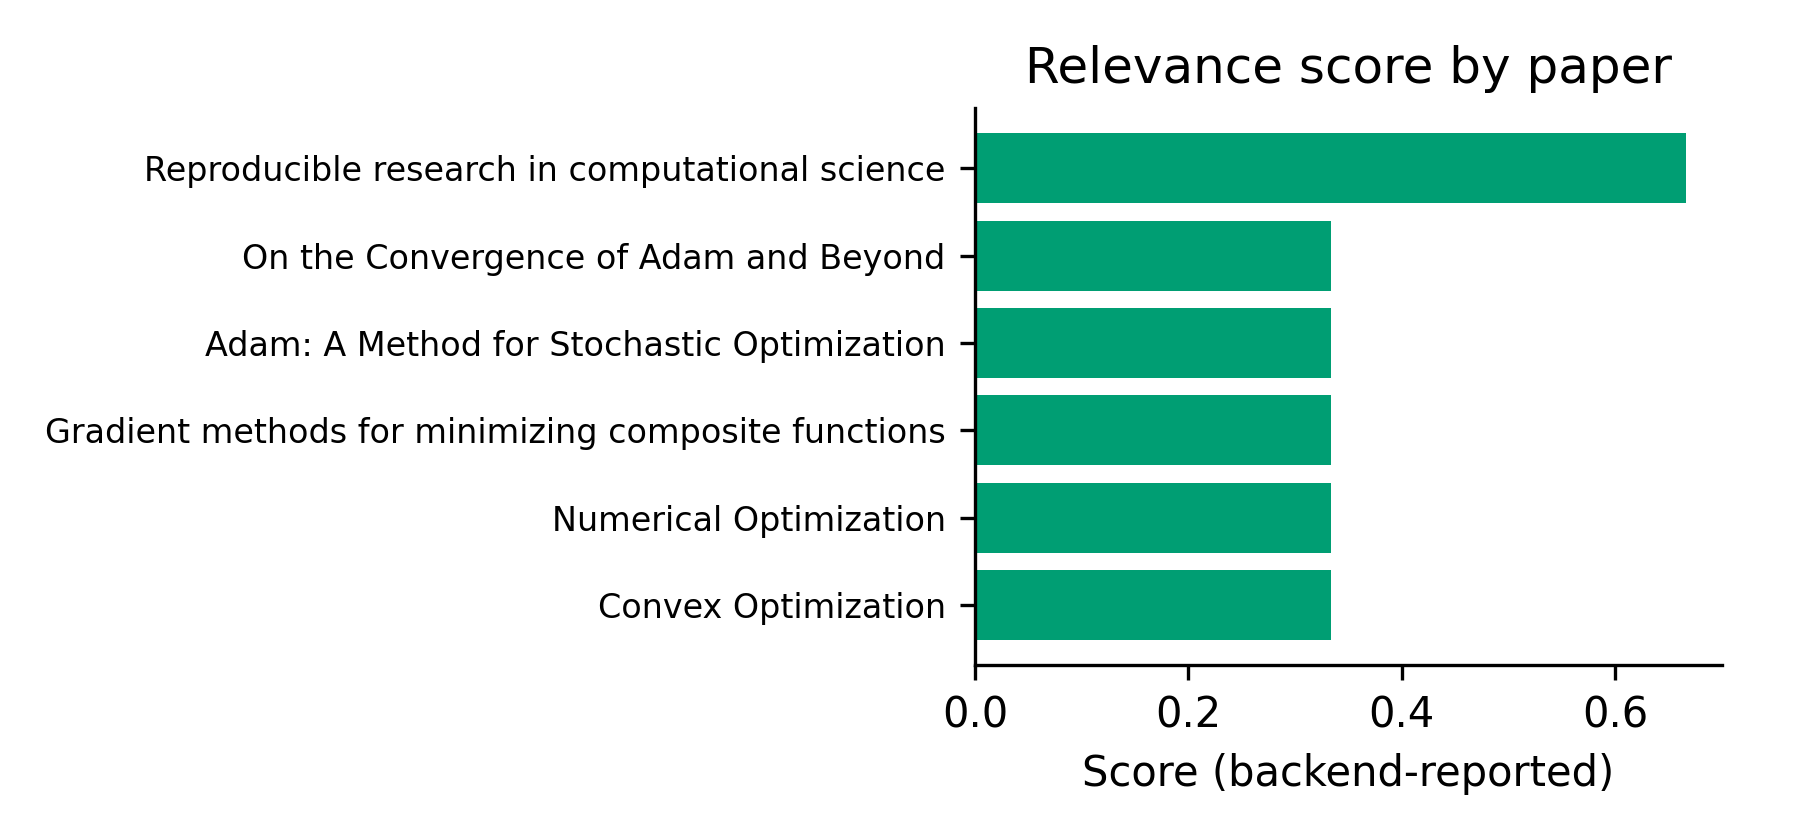
\includegraphics[keepaspectratio,alt={Per-paper backend-reported relevance scores ranked descending (highest at top). Each horizontal bar is one Paper.score; the y-tick label is the paper title truncated to 60 characters with an ellipsis. Backends without scoring (notably LocalBackend) report Paper.score = 0.0 so those bars have zero length. Generated by src/figures.py::plot\_score\_distribution.}]{../figures/score_distribution.png}}
\caption{Per-paper backend-reported relevance scores ranked descending
(highest at top). Each horizontal bar is one
\protect\texttt{Paper.score}; the y-tick label is the paper title
truncated to 60 characters with an ellipsis. Backends without scoring
(notably \protect\texttt{LocalBackend}) report
\protect\breaktt{Paper.score\ =\ 0.0} so those bars have zero length.
Generated by
\protect\breaktt{src/figures.py::plot\_score\_distribution}.}\label{fig:score_distribution}
\end{figure}

\newpage

\section{Results}\label{sec:results}

\textbf{Run snapshot.} With the bundled \breaktt{manuscript/config.yaml}
the most recent execution evaluated the query \emph{``reproducible
research optimization''} against local, returned 6 deduplicated paper(s)
(4 carrying a DOI, 6 carrying an abstract); the per-source breakdown is
local=6 and recorded backend errors are none. The deep-search workflow
(sec.~\ref{sec:deep_search}) covered 3 keyword(s) --- \emph{convex
optimization; stochastic gradient descent; reproducible research} ---
drawn from arxiv, crossref, paperclip, producing unique paper(s) after
cross-keyword deduplication.

The diagnostic figures generated for this run are catalogued in
sec.~\ref{sec:methodology}: fig.~\ref{fig:papers_per_source} surfaces
per-backend coverage, fig.~\ref{fig:year_histogram} surfaces the
temporal distribution, and fig.~\ref{fig:score_distribution} surfaces
the relevance-score profile. The full determinism contract for each
stage is itemised in tbl.~\ref{tbl:determinism} of
sec.~\ref{sec:reproducibility}.

\subsection{Interpreting the run
snapshot}\label{interpreting-the-run-snapshot}

The numerical values in the run-snapshot paragraph that opens this
section are read directly from \breaktt{output/run\_summary.json} and
\breaktt{output/data/manuscript\_variables.json} so they always reflect
the most recent run rather than a stale claim hand-typed into the prose.
Three properties are worth highlighting (the formal determinism contract
for each underlying stage is enumerated in tbl.~\ref{tbl:determinism}):

\begin{itemize}
\tightlist
\item
  \textbf{Cache reuse is observable.} A second invocation against the
  same config produces a byte-identical artifact tree (modulo the
  wall-clock timestamp inside
  \texttt{output/search/cache/search\_\textless{}hash\textgreater{}.json}
  itself); see also the \emph{Search (cached hit)} row of
  tbl.~\ref{tbl:determinism} and the verification recipe in
  sec.~\ref{sec:reproducibility}. The cache file thus doubles as a
  cryptographic seal: re-running is a file read, not a network
  round-trip.
\item
  \textbf{Deduplication is signal-preserving.} The aggregator merges by
  DOI \texorpdfstring{\ensuremath{\to}}{->} arXiv id \texorpdfstring{\ensuremath{\to}}{->} normalised (title, year), keeping the highest-scored
  copy and filling missing fields from the loser (see \emph{Dedup /
  merge} in tbl.~\ref{tbl:determinism} and the per-backend pre-dedup
  view in fig.~\ref{fig:papers_per_source}). The
  \breaktt{RESULT\_NUM\_PAPERS} figure therefore equals ``papers a
  reviewer needs to read'', not ``raw backend hit count'' --- the
  per-source contributions in \breaktt{RESULT\_PER\_SOURCE} are the
  pre-dedup view.
\item
  \textbf{Enrichment coverage is honest.}
  \breaktt{RESULT\_WITH\_ABSTRACT} and \texttt{RESULT\_WITH\_DOI} count
  fields the corpus or the \texttt{AbstractFetcher} actually populated,
  never values inferred. When a paper is missing a DOI it is excluded
  from the DOI count even if its arXiv id resolves to one upstream. The
  temporal coverage of those papers is summarised by
  fig.~\ref{fig:year_histogram}, and their backend-reported relevance
  scores by fig.~\ref{fig:score_distribution}.
\end{itemize}

\subsection{Output artefacts}\label{output-artefacts}

After running \breaktt{scripts/run\_search\_pipeline.py} against the
default \breaktt{manuscript/config.yaml}, the project produces:

\begin{itemize}
\tightlist
\item
  \breaktt{output/search/results.json} --- the raw \texttt{SearchResult}
  JSON, including \breaktt{per\_source\_counts} and \texttt{errors} for
  diagnostic purposes.
\item
  \texttt{output/search/cache/search\_\textless{}hash\textgreater{}.json}
  --- the deterministic search cache; identical reruns are file reads.
\item
  \texttt{output/cache/abs/\textless{}safe\_id\textgreater{}.txt} ---
  one file per fetched abstract.
\item
  \texttt{output/cache/pdf/\textless{}safe\_id\textgreater{}.\{pdf,txt\}}
  --- PDFs and extracted text (only when
  \breaktt{enrichment.fetch\_fulltext:\ true}).
\item
  \breaktt{output/corpus.json} --- a \texttt{LocalBackend}-compatible
  JSON corpus of every result, enriched in place.
\item
  \breaktt{manuscript/references.bib} --- the auto-populated bibliography
  from the single-query pipeline (merged with any other
  \breaktt{manuscript/*.bib} at PDF render time).
\item
  \texttt{output/llm/per\_paper/\textless{}safe\_id\textgreater{}.md}
  --- per-paper LLM analyses (only when \breaktt{llm.per\_paper:\ true}
  \emph{and} the LLM stack is reachable).
\item
  \breaktt{output/llm/synthesis.md} --- corpus-level LLM synthesis (only
  when \breaktt{llm.corpus\_synthesis:\ true} \emph{and} the LLM stack is
  reachable).
\item
  \breaktt{output/reading\_report.md} --- the final assembled reading
  report.
\end{itemize}

When the LLM stack is genuinely unreachable, the \texttt{output/llm/}
artefacts are simply absent --- no placeholder file is ever written into
the archive (see sec.~\ref{sec:pipeline_internals}).

Because the search cache and abstract cache are deterministic, a second
run with identical \texttt{config.yaml} produces byte-identical
artifacts (modulo timestamp metadata in the cache files themselves).
This is the property the project exists to demonstrate.

The exact paper count, DOI list, and synthesis text depend on the live
state of arXiv and Crossref at the time of the run --- and are therefore
not reproducible \emph{across} runs in different weeks. Users seeking
strict reproducibility should:

\begin{enumerate}
\def\labelenumi{\arabic{enumi}.}
\tightlist
\item
  Pin a \texttt{LocalBackend} corpus generated from a successful run
  (\breaktt{infrastructure.search.literature.write\_corpus}) and remove
  \texttt{arxiv} / \texttt{crossref} from
  \breaktt{config.search.sources}.
\item
  Commit the \breaktt{output/search/cache/} directory to version control.
\item
  Pin the LLM seed (\texttt{config.llm.seed}) and avoid model upgrades.
\end{enumerate}

With those three steps, every run from the same commit produces the same
outputs.

\newpage

\section{Conclusion}\label{sec:conclusion}

\breaktt{template\_search\_project} packages a complete, configurable,
reproducible literature workflow into the Research Project Template's
two-layer architecture. By keeping discovery, export, and synthesis in
three orthogonal infrastructure modules, the project demonstrates that
ambitious research automation can still respect the template's
principles:

\begin{itemize}
\tightlist
\item
  \textbf{Single source of truth} --- \texttt{Paper} for discovery,
  \texttt{BibEntry} for export, structured \texttt{SynthesisResult}
  records for LLM output.
\item
  \textbf{Test-driven development} --- every module is covered by
  real-data tests; HTTP backends are exercised through
  \breaktt{pytest-httpserver}, the LLM bridge through deterministic local
  callables.
\item
  \textbf{Thin orchestrator pattern} ---
  \breaktt{scripts/run\_search\_pipeline.py} does only argument parsing,
  configuration loading, and I/O; all logic lives in
  \texttt{infrastructure/} or \texttt{src/}.
\item
  \textbf{No mocks} --- neither in the new infrastructure modules nor in
  the project test suite.
\item
  \textbf{Multi-project support} --- the project lives alongside
  \breaktt{template\_code\_project/} and follows the same layout, so the
  existing pipeline runner discovers and executes it without
  modification.
\item
  \textbf{Reproducibility} --- deterministic search caching, on-disk
  enrichment caching, and pinned LLM seeds make a single
  \breaktt{manuscript/config.yaml} the only artifact a reviewer needs.
\end{itemize}

We close with three concrete extensions that build naturally on this
foundation:

\begin{enumerate}
\def\labelenumi{\arabic{enumi}.}
\tightlist
\item
  \textbf{Crossref TDM full-text fetch} for non-arXiv DOIs, completing
  the abstract-to-fulltext picture without changing the project's API.
\item
  \textbf{CSL-JSON export} alongside BibTeX, enabling Zotero / Mendeley
  / Pandoc-CSL workflows from the same \texttt{BibDatabase}.
\item
  \textbf{Vector recall on \texttt{LocalBackend}} for curated corpora
  exceeding about 1000 papers, gated behind an optional
  dependency.
\end{enumerate}

The infrastructure modules are deliberately small and stable; the
project that exercises them is deliberately small and explicit. Together
they show that \emph{domain-specific research automation} and
\emph{template-strict architectural discipline} are compatible --- and,
in fact, mutually reinforcing.

The bundled \breaktt{data/corpus.json} exercises classical optimisation
references
\citep{boyd2004convex, nocedal2006numerical, nesterov2013gradient}
alongside modern stochastic-optimisation work
\citep{kingma2014adam, reddi2018convergence} and the canonical
reproducibility paper \citep{peng2011reproducible}, so the
auto-generated \breaktt{manuscript/references.bib} always contains real
citation-ready entries that downstream tooling can resolve.

\newpage

\section{Pipeline Internals}\label{sec:pipeline_internals}

This supplemental section documents the data structures and on-disk
artifacts the pipeline produces, for readers who want to extend or audit
it.

\subsection{Data structures}\label{data-structures}

The Mermaid class diagram in this subsection shows the canonical fields
each record carries through the pipeline. Records have additional
optional metadata (e.g.~\texttt{Paper.url}, \texttt{Paper.publisher},
\texttt{Paper.isbn}, \texttt{Paper.raw}) omitted for readability ---
consult \breaktt{infrastructure/search/literature/models.py}
(\href{https://github.com/docxology/template/tree/main/infrastructure/search/literature}{source
on GitHub}) and \texttt{src/pipeline.py}
(\href{https://github.com/docxology/template/tree/main/projects/templates/template_search_project/src}{source
on GitHub}) for the full schema.

\begin{figure}[htbp]
\centering
\begin{verbatim}
classDiagram
    class SearchQuery {
        +str text
        +int max_results
        +int|None year_min
        +int|None year_max
        +list~str~ sources
        +list~str~ fields
        +matches_year(year) bool
    }

    class Paper {
        +str id
        +str title
        +list~str~ authors
        +int|None year
        +str|None doi
        +str|None url
        +str|None abstract
        +str|None pdf_url
        +str|None fulltext
        +str|None venue
        +str|None venue_type
        +str|None volume
        +str|None issue
        +str|None pages
        +str|None publisher
        +str|None edition
        +str|None isbn
        +list~str~ keywords
        +str|None source
        +float score
        +dict raw
        +to_dict() dict
        +from_dict(d) Paper
    }

    class SearchResult {
        +SearchQuery query
        +list~Paper~ papers
        +dict per_source_counts
        +dict errors
        +to_dict() dict
        +to_json() str
    }

    class BibEntry {
        +str entry_type
        +str citation_key
        +OrderedDict fields
    }

    class BibDatabase {
        +list~BibEntry~ entries
        +str|None preamble
        +find(key) BibEntry
    }

    class LiteratureRunArtifacts {
        +SearchResult result
        +Path|None corpus_path
        +Path|None bibtex_path
        +list~FetchResult~ enrichment_log
        +Path|None cache_dir
        +dict citation_keys
        +papers() list~Paper~
    }

    class ManuscriptVariables {
        +str config_query
        +int config_max_results
        +str config_sources
        +int result_num_papers
        +int result_num_sources
        +str result_per_source
        +str result_errors
        +str result_year_min
        +str result_year_max
        +int result_with_abstract
        +int result_with_doi
        +int deep_max_results_per_keyword
        +int deep_keyword_count
        +str deep_keywords_joined
        +str deep_sources
        +str deep_unique_papers
        +as_dict() dict
        +as_uppercase_keys() dict
    }

    class SynthesisResult {
        +str kind
        +str prompt
        +str text
        +str|None paper_id
    }

    SearchResult --> SearchQuery
    SearchResult --> "*" Paper
    LiteratureRunArtifacts --> SearchResult
    LiteratureRunArtifacts --> "*" BibEntry : via paper_to_bibentry
    BibDatabase --> "*" BibEntry
\end{verbatim}
\caption{Mermaid diagram}
\end{figure}

\subsection{On-disk layout}\label{on-disk-layout}

The project keeps committed input data in \texttt{data/}, regeneratable
outputs in \texttt{output/} (gitignored), and the manuscript source in
\texttt{manuscript/}. The Mermaid flowchart in this subsection (rendered
in the HTML build; the PDF build strips Mermaid) lists every artefact
the standard pipeline writes:

\begin{itemize}
\tightlist
\item
  \breaktt{data/corpus.json} --- the bundled offline corpus, CI-safe
  default for \texttt{LocalBackend}.
\item
  \breaktt{output/search/results.json} --- raw \texttt{SearchResult} JSON
  from the latest run.
\item
  \texttt{output/search/cache/search\_\textless{}hash\textgreater{}.json}
  --- deterministic \texttt{SearchCache} files.
\item
  \texttt{output/cache/abs/\textless{}safe\_id\textgreater{}.txt} ---
  one cached abstract per paper.
\item
  \texttt{output/cache/pdf/\textless{}safe\_id\textgreater{}.\{pdf,txt\}}
  --- PDF bytes plus extracted text.
\item
  \breaktt{output/llm/synthesis.md} --- corpus-level LLM synthesis (when
  enabled).
\item
  \texttt{output/llm/per\_paper/\textless{}safe\_id\textgreater{}.md}
  --- one per-paper note per paper (when enabled).
\item
  \texttt{../figures/\{papers\_per\_source,year\_histogram,score\_distribution\}.png}
  --- diagnostic figures.
\item
  \breaktt{output/data/manuscript\_variables.json} --- substitution table
  consumed by the resolver.
\item
  \breaktt{output/corpus.json} --- enriched corpus, written in
  \texttt{LocalBackend}-compatible format so it can re-seed a
  deterministic future run.
\item
  \breaktt{output/enrichment\_log.json} --- one entry per fetcher per
  paper.
\item
  \breaktt{output/reading\_report.md} --- final markdown reading report.
\item
  \breaktt{output/run\_summary.json} --- one-line metadata for the run.
\item
  \breaktt{manuscript/references.bib} --- auto-populated, Pandoc-ready
  BibTeX.
\end{itemize}

\begin{figure}[htbp]
\centering
\begin{verbatim}
flowchart TB
    P["projects/templates/template_search_project/"]
    P --> DAT["data/<br/>committed"]
    P --> OUT["output/<br/>regeneratable · gitignored"]
    P --> MAN["manuscript/"]

    DAT --> CORP_IN["corpus.json<br/>bundled offline corpus<br/>CI-safe default"]

    OUT --> SR["search/"]
    OUT --> CC["cache/"]
    OUT --> LD["llm/"]
    OUT --> FIG["figures/"]
    OUT --> DD["data/"]
    OUT --> CORP_OUT["corpus.json<br/>enriched · LocalBackend-compatible"]
    OUT --> ELOG["enrichment_log.json<br/>per-fetch status"]
    OUT --> RR[reading_report.md]
    OUT --> RS[run_summary.json]

    SR --> SR_R["results.json<br/>SearchResult"]
    SR --> SR_C["cache/search_HASH.json<br/>deterministic SearchCache"]

    CC --> CC_A["abs/SAFE_ID.txt"]
    CC --> CC_P["pdf/SAFE_ID.pdf and .txt"]

    LD --> LD_S[synthesis.md]
    LD --> LD_PP["per_paper/SAFE_ID.md"]

    FIG --> F1[papers_per_source.png]
    FIG --> F2[year_histogram.png]
    FIG --> F3[score_distribution.png]

    DD --> MV[manuscript_variables.json]

    MAN --> BIB["references.bib<br/>auto-populated · Pandoc-ready"]

    classDef dir fill:#0f172a,stroke:#0f172a,color:#fff
    classDef gen fill:#0f766e,stroke:#0f172a,color:#fff
    classDef src fill:#1e3a8a,stroke:#0f172a,color:#fff
    class P,DAT,OUT,MAN,SR,CC,LD,FIG,DD dir
    class CORP_OUT,ELOG,RR,RS,SR_R,SR_C,CC_A,CC_P,LD_S,LD_PP,F1,F2,F3,MV,BIB gen
    class CORP_IN src
\end{verbatim}
\caption{Mermaid diagram}
\end{figure}

\subsection{Citation-key collision
handling}\label{citation-key-collision-handling}

\breaktt{paper\_to\_bibentry()} generates citation keys as
\texttt{\textless{}author\textgreater{}\textless{}year\textgreater{}\textless{}title-word\textgreater{}}
(with stop-words filtered and unicode folded). When two papers in the
same result set produce the same key --- common when one author
publishes multiple papers in the same year on closely related topics ---
\breaktt{src/pipeline.py::\_disambiguate\_citation\_key} appends a
deterministic suffix from the alphabet (\texttt{a}, \texttt{b}, \ldots,
\texttt{z}, then two-letter combinations \texttt{aa}, \texttt{ab},
\ldots) until uniqueness is restored, with a numeric \texttt{\_1},
\texttt{\_2}, \ldots{} fallback for the pathological case. The mapping
is exposed to downstream stages via
\breaktt{LiteratureRunArtifacts.citation\_keys}, and the report uses
these keys verbatim, so the LLM synthesis and the BibTeX file always
agree.

The deep-search workflow has its own collision handler in
\breaktt{src/deep\_search.py::run\_deep\_search} that operates over the
post-deduplication aggregate roster --- see sec.~\ref{sec:deep_search}
--- and the unified \breaktt{references\_deep.bib} reflects the same
mapping.

\subsection{Failure isolation}\label{failure-isolation}

\begin{itemize}
\tightlist
\item
  \textbf{A backend is unreachable.} \breaktt{LiteratureClient} records
  the message into \texttt{result.errors{[}name{]}} and continues. The
  reading report surfaces these errors in a callout block at the top.
\item
  \textbf{An abstract fetch fails.} The fetcher records
  \texttt{status="error"} in \breaktt{enrichment\_log.json} and the paper
  keeps its existing (possibly empty) abstract.
\item
  \textbf{A PDF fetch fails or \texttt{pypdf} is missing.} Same pattern
  --- the PDF, if downloaded, is still cached on disk. The reading
  report does not reference the missing fulltext.
\item
  \textbf{The LLM is unreachable or unconfigured.}
  \breaktt{scripts/run\_search\_pipeline.py} logs a warning and skips the
  synthesis stage entirely --- \texttt{output/llm/} is left empty and
  the reading report omits both the per-paper-notes and cross-corpus
  sections. No placeholder text is ever written into the archive, so a
  missing LLM is observable from the absence of those sections rather
  than from a fake ``(LLM unavailable)'' string.
\end{itemize}

\newpage

\section{Reproducibility}\label{sec:reproducibility}

Reproducibility in computational research has well-documented
prerequisites: open data, open code, and a deterministic build that can
be re-run from scratch \citep{peng2011reproducible}. The bundled
\breaktt{manuscript/config.yaml} is intentionally configured to satisfy
all three for \textbf{strict reproducibility}:

\begin{enumerate}
\def\labelenumi{\arabic{enumi}.}
\tightlist
\item
  \texttt{search.sources:\ {[}local{]}} consumes
  \breaktt{data/corpus.json}, which is a curated and committed JSON
  corpus. No network is required to run the pipeline.
\item
  \breaktt{search.cache\_dir:\ output/search/cache} writes deterministic
  JSON cache files; running the same query twice produces a
  byte-identical artifact tree (modulo timestamp metadata in the cache
  file itself).
\item
  \breaktt{enrichment.fetch\_abstracts:\ true} reads abstracts directly
  from the corpus when present; no network fetch is required.
\item
  \breaktt{enrichment.fetch\_fulltext:\ false} is the default ---
  full-text fetching is opt-in and gated behind the optional
  \texttt{pypdf} dependency (\breaktt{uv\ sync\ -\/-group\ rendering}).
\item
  \breaktt{llm.enabled:\ false} is the default --- the LLM stage is
  opt-in and requires a running \texttt{ollama\ serve}. When enabled,
  \texttt{seed:\ 42} and \breaktt{temperature:\ 0.0} are pinned.
\end{enumerate}

\subsection{Switching to live search}\label{switching-to-live-search}

Replace the \texttt{sources} list with the desired backend set:

\begin{Shaded}
\begin{Highlighting}[]
\FunctionTok{search}\KeywordTok{:}
\AttributeTok{  }\FunctionTok{query}\KeywordTok{:}\AttributeTok{ }\StringTok{"your topic"}
\AttributeTok{  }\FunctionTok{sources}\KeywordTok{:}\AttributeTok{ }\KeywordTok{[}\AttributeTok{arxiv}\KeywordTok{,}\AttributeTok{ crossref}\KeywordTok{]}
\AttributeTok{  }\FunctionTok{crossref\_mailto}\KeywordTok{:}\AttributeTok{ }\StringTok{"you@example.org"}
\end{Highlighting}
\end{Shaded}

A first live run populates \breaktt{output/search/cache/}. Commit that
directory to the repo and the pipeline becomes reproducible across
machines without further configuration changes.

\subsection{Determinism guarantees}\label{determinism-guarantees}

The full determinism contract is itemised in tbl.~\ref{tbl:determinism}:
every pipeline stage is annotated as fully, conditionally, or
non-deterministic, with an explicit mechanism column so reviewers can
audit each row independently.

\begin{longtable}[]{@{}
  >{\raggedright\arraybackslash}p{(\linewidth - 4\tabcolsep) * \real{0.3333}}
  >{\raggedright\arraybackslash}p{(\linewidth - 4\tabcolsep) * \real{0.3333}}
  >{\raggedright\arraybackslash}p{(\linewidth - 4\tabcolsep) * \real{0.3333}}@{}}
\caption{Determinism contract by pipeline stage. Cached stages are
byte-stable across reruns; live stages depend on the upstream source and
are pinned to the cache file once a successful run
completes.}\label{tbl:determinism}\tabularnewline
\toprule\noalign{}
\begin{minipage}[b]{\linewidth}\raggedright
Stage
\end{minipage} & \begin{minipage}[b]{\linewidth}\raggedright
Deterministic?
\end{minipage} & \begin{minipage}[b]{\linewidth}\raggedright
Mechanism
\end{minipage} \\
\midrule\noalign{}
\endfirsthead
\toprule\noalign{}
\begin{minipage}[b]{\linewidth}\raggedright
Stage
\end{minipage} & \begin{minipage}[b]{\linewidth}\raggedright
Deterministic?
\end{minipage} & \begin{minipage}[b]{\linewidth}\raggedright
Mechanism
\end{minipage} \\
\midrule\noalign{}
\endhead
\bottomrule\noalign{}
\endlastfoot
Search (cached hit) & yes & \texttt{SearchCache} JSON files \\
Search (cache miss) & no & live API \\
Dedup / merge & yes & DOI / arXiv-id canonical keys; tie-break by score
then year \\
Citation-key generation & yes & unicode folding + stop-word skip;
collision suffix is deterministic \\
BibTeX writer & yes & byte-stable format pinning (verified by
\breaktt{tests/infra\_tests/reference/}) \\
Abstract fetch & yes (cached) / no (live) & per-paper
\texttt{\textless{}safe\_id\textgreater{}.txt} cache \\
Fulltext fetch & yes (cached) / mostly (live) & per-paper
\texttt{\textless{}safe\_id\textgreater{}.\{pdf,txt\}} cache; live
fetch's \texttt{pypdf} text extraction is not bit-stable across
versions \\
LLM synthesis & mostly & \texttt{seed=42}, \texttt{temperature=0.0};
Ollama deterministic up to its own minor variance \\
Figure generation & yes (within Matplotlib version) & fixed palette,
fixed bin width, no random subsampling \\
\end{longtable}

\subsection{Verifying reproducibility
locally}\label{verifying-reproducibility-locally}

\begin{Shaded}
\begin{Highlighting}[]
\CommentTok{\# Run twice; nothing in output/ should diff except the cache timestamps.}
\ExtensionTok{uv}\NormalTok{ run python projects/templates/template\_search\_project/scripts/run\_search\_pipeline.py}
\FunctionTok{mv}\NormalTok{ projects/templates/template\_search\_project/output projects/templates/template\_search\_project/output\_first}
\ExtensionTok{uv}\NormalTok{ run python projects/templates/template\_search\_project/scripts/run\_search\_pipeline.py}
\FunctionTok{diff} \AttributeTok{{-}ru} \DataTypeTok{\textbackslash{}}
\NormalTok{    projects/templates/template\_search\_project/output\_first/corpus.json }\DataTypeTok{\textbackslash{}}
\NormalTok{    projects/templates/template\_search\_project/output/corpus.json}
\end{Highlighting}
\end{Shaded}

The only expected differences are inside
\breaktt{output/search/cache/search\_*.json}, where \texttt{\_cached\_at}
is wall-clock time at write.

\subsection{Limitations}\label{limitations}

The reproducibility contract enumerated in
sec.~\ref{sec:reproducibility} (items 1--5 and
tbl.~\ref{tbl:determinism}) does not eliminate the following
well-defined sources of non-reproducibility, which are surfaced here so
reviewers can audit them explicitly rather than inferring from the
contract table:

\begin{itemize}
\tightlist
\item
  \textbf{Live search drift.} When \breaktt{config.search.sources}
  includes \texttt{arxiv} or \texttt{crossref}, the first cache-miss
  invocation hits the live API; the cached JSON freezes that response,
  but two cold-start clones running on different days will see different
  paper sets. Pin a \texttt{LocalBackend} corpus or commit
  \breaktt{output/search/cache/} to break this dependency.
\item
  \textbf{\texttt{pypdf} version drift.} The fulltext fetcher uses
  \texttt{pypdf} to extract text from a downloaded PDF. \texttt{pypdf}'s
  text-extraction algorithm is not bit-stable across major versions;
  upgrading \texttt{pypdf} can produce different
  \texttt{\textless{}safe\_id\textgreater{}.txt} cache contents from the
  same source PDF. The PDF bytes themselves are bit-stable so the cache
  freezes the inputs, not the extraction.
\item
  \textbf{Ollama version drift.} Pinning \texttt{seed=42} and
  \texttt{temperature=0.0} controls Ollama's sampling, but the model
  weights, tokenizer, and template can change between Ollama releases.
  Document the Ollama version alongside \breaktt{config.llm.model} when
  archiving a run for replication.
\item
  \textbf{Paperclip backend status.} The \texttt{paperclip} backend is
  opt-in and currently degrades to HTTP 405 on the production endpoint;
  the run records the error in
  \texttt{SearchResult.errors{[}paperclip{]}} and continues. Treat
  \texttt{paperclip} results as advisory until the upstream service
  stabilises.
\item
  \textbf{External backend behaviour outside this project's control.}
  arXiv and Crossref are the source of truth; this project is faithful
  to whatever they return. A retraction, metadata fix, or DOI assignment
  upstream will alter the cache on the next cold-start invocation.
\end{itemize}

These limitations bound \emph{what} the cache + seed + corpus pinning
achieves. Inside those bounds, the contract in
tbl.~\ref{tbl:determinism} is total: every cached pipeline stage is
byte-stable across reruns (verified by
\breaktt{tests/test\_pipeline.py::TestRunLiteraturePipeline::test\_bibtex\_byte\_identical\_across\_reruns}).

\newpage

\section{Deep Search}\label{sec:deep_search}

The deep-search workflow extends the standard literature pipeline along
three axes: \textbf{breadth} (multi-keyword fan-out), \textbf{depth}
(full enrichment of every paper, abstract + PDF fulltext), and
\textbf{archival quality} (per-paper multi-section LLM reading notes
saved as standalone markdown). It is invoked from the same configuration
file but a separate orchestrator script.

\subsection{Configuration}\label{configuration}

The \texttt{deep\_search:} block in \breaktt{manuscript/config.yaml}
controls the run. The most-used knobs:

\begin{itemize}
\tightlist
\item
  \texttt{keywords} --- list of free-text queries (each becomes one
  \texttt{SearchQuery}).
\item
  \breaktt{max\_results\_per\_keyword} --- per-keyword cap (100 by
  default; honoured by the aggregator after dedup).
\item
  \texttt{sources} --- backend list, same vocabulary as the standard
  pipeline (\texttt{arxiv}, \texttt{crossref}, \texttt{local},
  \texttt{paperclip}).
\item
  \texttt{fetch\_abstracts} / \texttt{fetch\_fulltext} --- when both are
  \texttt{true}, every returned paper has its abstract fetched (arXiv
  export API) and (where a PDF URL is available) its fulltext extracted
  via \texttt{pypdf}. Cached on disk under \breaktt{output/cache/abs/}
  and \breaktt{output/cache/pdf/}.
\item
  \texttt{llm\_per\_paper} --- when \texttt{true} and Ollama is
  reachable, each paper gets a multi-section markdown reading note
  generated by the local LLM. When \texttt{false}, or when the LLM stack
  is genuinely unreachable at runtime, the per-paper note is written
  with only the abstract / fulltext-excerpt sections; the synthesis
  section is omitted entirely (no placeholder text). The composer's
  Supplemental S1 also drops the per-paper synthesis subsection in that
  case rather than emitting empty rows.
\item
  \breaktt{write\_unified\_bibtex} / \breaktt{unified\_bibtex\_path} ---
  when \texttt{true}, a deduplicated, collision-suffixed BibTeX file is
  written under \breaktt{manuscript/references\_deep.bib} so it can be
  cited from the manuscript via Pandoc \texttt{{[}@key{]}} syntax
  exactly the same way as the hand-curated \texttt{references.bib}.
\end{itemize}

\subsection{Pipeline shape}\label{pipeline-shape}

The deep-search pipeline reads the \texttt{deep\_search:} block from
\breaktt{manuscript/config.yaml}, runs one \texttt{SearchQuery} per
keyword (capped at \breaktt{max\_results\_per\_keyword}), aggregates the
per-backend results through \breaktt{LiteratureClient}, enriches every
paper via \texttt{AbstractFetcher} and \texttt{FulltextFetcher},
generates collision-free citation keys with
\breaktt{paper\_to\_bibentry}, and (when \breaktt{llm\_per\_paper:\ true}
and Ollama is reachable) calls the local LLM with \texttt{DEEP\_PROMPT}
to produce a seven-section reading note per paper. The per-keyword
outputs are then merged by \texttt{merge\_papers} to form a deduplicated
aggregate roster which is written to
\breaktt{manuscript/references\_deep.bib},
\breaktt{output/deep\_search/aggregate.json}, and
\breaktt{output/deep\_search/aggregate\_report.md}. A Mermaid flowchart
in this subsection renders the same flow visually in the HTML build.

\begin{figure}[htbp]
\centering
\begin{verbatim}
flowchart TB
    CFG[deep_search block of config.yaml]
    CFG --> KW{{For each keyword}}
    KW --> SEARCH[SearchQuery · max_results_per_keyword]
    SEARCH --> CLIENT["LiteratureClient<br/>aggregates arxiv · crossref · local · paperclip"]
    CLIENT --> ENRICH["AbstractFetcher + FulltextFetcher<br/>cached on disk"]
    ENRICH --> KEYS["paper_to_bibentry<br/>collision-free keys"]
    KEYS --> LLMQ{LLM per-paper?}
    LLMQ -- yes --> LLM["Ollama LLMClient<br/>DEEP_PROMPT · 7 sections"]
    LLMQ -- no --> SKIP[skip synthesis · no placeholder]
    LLM --> NOTE[output/deep_search/&lt;slug&gt;/per_paper/&lt;safe_id&gt;.md]
    SKIP --> NOTE
    NOTE --> KR[KeywordResult]

    KR --> AGG[merge_papers across all keywords]
    AGG --> BIB["unified BibTeX<br/>references_deep.bib"]
    AGG --> AJSON[aggregate.json]
    AGG --> AMD[aggregate_report.md]

    classDef cfg fill:#0f172a,stroke:#0f172a,color:#fff
    classDef proc fill:#1e3a8a,stroke:#0f172a,color:#fff
    classDef llm fill:#7c2d12,stroke:#0f172a,color:#fff
    classDef out fill:#0f766e,stroke:#0f172a,color:#fff
    class CFG,KW,LLMQ cfg
    class SEARCH,CLIENT,ENRICH,KEYS,KR,AGG proc
    class LLM,SKIP llm
    class NOTE,BIB,AJSON,AMD out
\end{verbatim}
\caption{Mermaid diagram}
\end{figure}

\subsection{LLM prompt}\label{llm-prompt}

The deep-search prompt is richer than the standard
\breaktt{synthesis.PROMPT\_PER\_PAPER}. It produces a self-contained
reading note suitable for archival without re-reading the paper:

\begin{verbatim}
## Contribution
One paragraph stating the paper's central claim and why it is novel.

## Method
2-4 bullets describing the technical approach.

## Evidence
2-4 bullets describing experiments / proofs.

## Limitations
1-3 bullets covering caveats and what the paper does NOT address.

## Connections
1-3 bullets relating this paper to other work in the field, citing only
papers explicitly named in the input.

## Significance for {keyword}
One paragraph explaining why this paper matters for the keyword.

## Tags
5-10 lowercase keywords.
\end{verbatim}

The LLM is duck-typed as \texttt{Callable{[}{[}str{]},\ str{]}} so tests
pass a deterministic local callable that returns real, well-formed
reading-note text; runtime callers wrap an
\breaktt{infrastructure.llm.LLMClient} with
\breaktt{seed=42,\ temperature=0.0} for reproducibility. When the LLM
stack is unreachable, callers pass \texttt{None} and the per-paper
synthesis stage is skipped entirely --- no placeholder text is ever
written into the archive.

\subsection{On-disk layout}\label{on-disk-layout-1}

A successful deep-search run writes the following artefacts (paths shown
relative to the project root); a Mermaid tree in this subsection renders
the same hierarchy in the HTML build:

\begin{itemize}
\tightlist
\item
  \breaktt{output/deep\_search/aggregate.json} --- every unique paper
  across keywords.
\item
  \breaktt{output/deep\_search/aggregate\_report.md} --- cross-keyword
  markdown summary.
\item
  \breaktt{output/deep\_search/run\_summary.json} --- one-line metadata
  for the run.
\item
  \texttt{output/deep\_search/\textless{}keyword\_slug\textgreater{}/papers.json}
  --- enriched per-keyword paper list.
\item
  \texttt{output/deep\_search/\textless{}keyword\_slug\textgreater{}/reading\_report.md}
  --- per-keyword markdown summary.
\item
  \texttt{output/deep\_search/\textless{}keyword\_slug\textgreater{}/per\_paper/\textless{}safe\_id\textgreater{}.md}
  --- one reading note per paper.
\item
  \breaktt{manuscript/references\_deep.bib} --- auto-generated,
  deduplicated unified BibTeX file.
\end{itemize}

\begin{figure}[htbp]
\centering
\begin{verbatim}
flowchart TB
    P["projects/templates/template_search_project/"]
    P --> OUT["output/deep_search/"]
    P --> BIB["manuscript/references_deep.bib<br/>auto-generated · deduplicated"]

    OUT --> AGG["aggregate.json<br/>every unique paper"]
    OUT --> AMD["aggregate_report.md<br/>cross-keyword summary"]
    OUT --> RS["run_summary.json<br/>one-line metadata"]
    OUT --> KW1["&lt;keyword_slug_1&gt;/"]
    OUT --> KW2["&lt;keyword_slug_2&gt;/"]
    OUT --> KW3["&lt;keyword_slug_3&gt;/"]

    KW1 --> KW1_P[papers.json]
    KW1 --> KW1_R[reading_report.md]
    KW1 --> KW1_PP["per_paper/<br/>SAFE_ID.md per paper"]

    classDef d fill:#0f172a,stroke:#0f172a,color:#fff
    classDef f fill:#0f766e,stroke:#0f172a,color:#fff
    classDef bib fill:#1e3a8a,stroke:#0f172a,color:#fff
    class P,OUT,KW1,KW2,KW3,KW1_PP d
    class AGG,AMD,RS,KW1_P,KW1_R f
    class BIB bib
\end{verbatim}
\caption{Mermaid diagram}
\end{figure}

\subsection{Determinism}\label{determinism}

Three caches make this workflow replayable:

\begin{enumerate}
\def\labelenumi{\arabic{enumi}.}
\tightlist
\item
  \texttt{SearchCache}
  (\texttt{output/search/cache/search\_\textless{}hash\textgreater{}.json})
  --- keyed on canonical query identity per keyword.
\item
  Abstract cache
  (\texttt{output/cache/abs/\textless{}safe\_id\textgreater{}.txt}).
\item
  Fulltext cache
  (\texttt{output/cache/pdf/\textless{}safe\_id\textgreater{}.\{pdf,txt\}}).
\item
  LLM seed (\breaktt{deep\_search.llm\_seed:\ 42}) + temperature
  (\texttt{0.0}).
\end{enumerate}

Commit any subset of these caches to version control to freeze a run.

\subsection{Paperclip backend}\label{paperclip-backend}

The \href{https://paperclip.gxl.ai}{Paperclip backend} is opt-in. Enable
it by:

\begin{enumerate}
\def\labelenumi{\arabic{enumi}.}
\tightlist
\item
  Creating \breaktt{projects/templates/template\_search\_project/.env}
  (gitignored) with your \breaktt{PAPERCLIP\_API\_KEY=gxl\_…} (template
  at \texttt{.env.example}).
\item
  Including \texttt{paperclip} in \breaktt{deep\_search.sources}.
\end{enumerate}

The orchestrator scripts auto-load \texttt{.env} via the lightweight
\texttt{src.dotenv} module before constructing the backend list. The
\breaktt{PaperclipBackend} adapter mirrors the wire protocol of the
official \texttt{gxl\_paperclip} Python SDK: \texttt{POST\ /papers} with
an \texttt{X-API-Key} header and a JSON-RPC \texttt{tools/call}
envelope. We support both the modern \breaktt{structuredContent.papers}
response shape and the older text-only \texttt{content{[}{]}.text} shape
(best-effort regex extraction).

Failure-isolation: any per-backend error (including the migration-state
HTTP 405 the production endpoint may currently return) is captured into
\texttt{SearchResult.errors{[}paperclip{]}} and the run continues. See
\texttt{output/deep\_search/\textless{}keyword\textgreater{}/papers.json}
and the aggregate \breaktt{run\_summary.json} for the recorded errors.

\subsection{CLI}\label{cli}

\begin{Shaded}
\begin{Highlighting}[]
\CommentTok{\# Run with everything from config.yaml (assumes deep\_search.enabled: true)}
\ExtensionTok{uv}\NormalTok{ run python projects/templates/template\_search\_project/scripts/run\_deep\_search.py}

\CommentTok{\# Force{-}enable without touching config.yaml}
\ExtensionTok{uv}\NormalTok{ run python projects/templates/template\_search\_project/scripts/run\_deep\_search.py }\AttributeTok{{-}{-}enable}

\CommentTok{\# Override keyword list at the command line}
\ExtensionTok{uv}\NormalTok{ run python projects/templates/template\_search\_project/scripts/run\_deep\_search.py }\DataTypeTok{\textbackslash{}}
    \AttributeTok{{-}{-}enable} \AttributeTok{{-}{-}keyword} \StringTok{"convex optimization"} \AttributeTok{{-}{-}keyword} \StringTok{"stochastic gradient descent"}

\CommentTok{\# Skip LLM stage even when config enables it}
\ExtensionTok{uv}\NormalTok{ run python projects/templates/template\_search\_project/scripts/run\_deep\_search.py }\AttributeTok{{-}{-}enable} \AttributeTok{{-}{-}no{-}llm}

\CommentTok{\# Bypass cache (writes still happen)}
\ExtensionTok{uv}\NormalTok{ run python projects/templates/template\_search\_project/scripts/run\_deep\_search.py }\AttributeTok{{-}{-}enable} \AttributeTok{{-}{-}no{-}cache}

\CommentTok{\# Local{-}corpus mode (offline · CI{-}friendly)}
\ExtensionTok{uv}\NormalTok{ run python projects/templates/template\_search\_project/scripts/run\_deep\_search.py }\DataTypeTok{\textbackslash{}}
    \AttributeTok{{-}{-}enable} \AttributeTok{{-}{-}corpus}\NormalTok{ projects/templates/template\_search\_project/data/corpus.json}
\end{Highlighting}
\end{Shaded}

\newpage

\newpage

\section{Supplemental S1 --- Literature Review (auto-composed from deep
search)}\label{sec:supplemental_s1}

\emph{Composed by \breaktt{scripts/s\_compose\_literature\_review.py}
from the most recent deep-search run. Edit the script, not this file ---
manual edits will be overwritten on the next pipeline run.}

This review covers \textbf{3 keyword(s)}, \textbf{300 unique paper(s)}
(retrieved at up to 100 per keyword from arxiv, crossref, paperclip).
All references are stored in \breaktt{manuscript/references\_deep.bib}
and resolved by the combined-PDF pipeline (Pandoc \texttt{-\/-natbib} +
BibTeX over all \breaktt{manuscript/*.bib} files).

\subsection{convex optimization}\label{convex-optimization}

\emph{Papers retrieved:} \textbf{100} \texorpdfstring{\ensuremath{\cdot}}{.} \emph{per-source contributions:}
arxiv=100, crossref=100, paperclip=95 \texorpdfstring{\ensuremath{\cdot}}{.} \emph{backend errors:} none

{\def\LTcaptype{none} % do not increment counter
\begin{longtable}[]{@{}
  >{\raggedright\arraybackslash}p{(\linewidth - 6\tabcolsep) * \real{0.2308}}
  >{\raggedright\arraybackslash}p{(\linewidth - 6\tabcolsep) * \real{0.2308}}
  >{\raggedleft\arraybackslash}p{(\linewidth - 6\tabcolsep) * \real{0.3077}}
  >{\raggedright\arraybackslash}p{(\linewidth - 6\tabcolsep) * \real{0.2308}}@{}}
\toprule\noalign{}
\begin{minipage}[b]{\linewidth}\raggedright
Cite
\end{minipage} & \begin{minipage}[b]{\linewidth}\raggedright
Title
\end{minipage} & \begin{minipage}[b]{\linewidth}\raggedleft
Year
\end{minipage} & \begin{minipage}[b]{\linewidth}\raggedright
DOI / URL
\end{minipage} \\
\midrule\noalign{}
\endhead
\bottomrule\noalign{}
\endlastfoot
\citep{anon2004convex} & Convex optimization problems & 2004 & DOI
10.1017/cbo9780511804441.005
(\href{https://doi.org/10.1017/cbo9780511804441.005}{open}) \\
\citep{anon2004convexa} & Convex functions & 2004 & DOI
10.1017/cbo9780511804441.004
(\href{https://doi.org/10.1017/cbo9780511804441.004}{open}) \\
\citep{anonreverse} & Reverse Convex Optimization, Reverse convex
programming & n.d. & DOI 10.1007/springerreference\_72642
(\href{https://doi.org/10.1007/springerreference_72642}{open}) \\
\citep{anon2021convex} & Convex Optimization and Efficiency & 2021 & DOI
10.1017/9781108699211.006
(\href{https://doi.org/10.1017/9781108699211.006}{open}) \\
\citep{suh20221} & 1. Convex Optimization Basics & 2022 & DOI
10.1561/9781638280538.ch1
(\href{https://doi.org/10.1561/9781638280538.ch1}{open}) \\
\citep{anon2021ellipsoid} & Ellipsoid Method for Convex Optimization &
2021 & DOI 10.1017/9781108699211.015
(\href{https://doi.org/10.1017/9781108699211.015}{open}) \\
\citep{nesterov2004smooth} & Smooth Convex Optimization & 2004 & DOI
10.1007/978-1-4419-8853-9\_2
(\href{https://doi.org/10.1007/978-1-4419-8853-9_2}{open}) \\
\citep{nesterov2004nonsmooth} & Nonsmooth Convex Optimization & 2004 &
DOI 10.1007/978-1-4419-8853-9\_3
(\href{https://doi.org/10.1007/978-1-4419-8853-9_3}{open}) \\
\citep{anon2022convex} & Convex Optimization Basics & 2022 & DOI
10.1561/978-1-63828-053-820251002
(\href{https://doi.org/10.1561/978-1-63828-053-820251002}{open}) \\
\citep{anon2004convexb} & Convex sets & 2004 & DOI
10.1017/cbo9780511804441.003
(\href{https://doi.org/10.1017/cbo9780511804441.003}{open}) \\
\citep{anon2011what} & What Is Convex Optimization? & 2011 & DOI
10.1201/b11156-7 (\href{https://doi.org/10.1201/b11156-7}{open}) \\
\citep{anon2011convex} & Convex Semi-Infinite Optimization & 2011 & DOI
10.1201/b11156-17 (\href{https://doi.org/10.1201/b11156-17}{open}) \\
\citep{anon2011tools} & Tools for Convex Optimization & 2011 & DOI
10.1201/b11156-8 (\href{https://doi.org/10.1201/b11156-8}{open}) \\
\citep{anon2004convexc} & Convex Sets. Convex and Generalized Convex
Functions & 2004 & DOI 10.1016/b978-044450550-7/50002-8
(\href{https://doi.org/10.1016/b978-044450550-7/50002-8}{open}) \\
\citep{anon20146} & 6 Convex optimization algorithms & 2014 & DOI
10.1515/9783110361629.117
(\href{https://doi.org/10.1515/9783110361629.117}{open}) \\
\citep{jacobsen2008reverse} & Reverse Convex Optimization & 2008 & DOI
10.1007/978-0-387-74759-0\_564
(\href{https://doi.org/10.1007/978-0-387-74759-0_564}{open}) \\
\citep{nesterov2018nonsmooth} & Nonsmooth Convex Optimization & 2018 &
DOI 10.1007/978-3-319-91578-4\_3
(\href{https://doi.org/10.1007/978-3-319-91578-4_3}{open}) \\
\citep{jacobsen2001bb} & \texorpdfstring{\ensuremath{\alpha}}{alpha}BB algorithm; Concave programming; D.C.
programming; Quadratic knapsack. Quadratic programming with bound
constraints; Reverse convex optimization Standard quadratic optimization
problems: Theory REVERSE CONVEX OPTIMIZATION & 2001 & DOI
10.1007/0-306-48332-7\_431
(\href{https://doi.org/10.1007/0-306-48332-7_431}{open}) \\
\citep{tuypartly} & Partly Convex and Convex-Monotonic Optimization
Problems & n.d. & DOI 10.1007/3-540-27170-8\_37
(\href{https://doi.org/10.1007/3-540-27170-8_37}{open}) \\
\citep{nesterov2018smooth} & Smooth Convex Optimization & 2018 & DOI
10.1007/978-3-319-91578-4\_2
(\href{https://doi.org/10.1007/978-3-319-91578-4_2}{open}) \\
\citep{anon2011weak} & Weak Sharp Minima in Convex Optimization & 2011 &
DOI 10.1201/b11156-15
(\href{https://doi.org/10.1201/b11156-15}{open}) \\
\citep{anonconvex} & Convex Discrete Optimization & n.d. & DOI
10.1007/springerreference\_72172
(\href{https://doi.org/10.1007/springerreference_72172}{open}) \\
\citep{anon2025convex} & Convex Functions & 2025 & DOI
10.1017/9781009510561.012
(\href{https://doi.org/10.1017/9781009510561.012}{open}) \\
\citep{zaslavski2020nonsmooth} & Nonsmooth Convex Optimization & 2020 &
DOI 10.1007/978-3-030-60300-7\_2
(\href{https://doi.org/10.1007/978-3-030-60300-7_2}{open}) \\
\citep{anon2020appendix} & Appendix: & 2020 & DOI 10.2307/j.ctvqsdxqd.15
(\href{https://doi.org/10.2307/j.ctvqsdxqd.15}{open}) \\
\citep{anon2005connectedness} & Connectedness of efficient points in
convex and convex transformable vector optimization & 2005 & DOI
10.1080/02331930500096270
(\href{https://doi.org/10.1080/02331930500096270}{open}) \\
\citep{anon2025convexa} & Convex Programming Problems and Convex Theorem
of the Alternative & 2025 & DOI 10.1017/9781009510561.021
(\href{https://doi.org/10.1017/9781009510561.021}{open}) \\
\citep{anon2011toolsa} & Tools for Convex Optimization & 2011 & DOI
10.1201/b11156-3 (\href{https://doi.org/10.1201/b11156-3}{open}) \\
\citep{tuy1998convex} & Convex Functions & 1998 & DOI
10.1007/978-1-4757-2809-5\_2
(\href{https://doi.org/10.1007/978-1-4757-2809-5_2}{open}) \\
\citep{mattingley2009automatic} & Automatic code generation for
real-time convex optimization & 2009 & DOI 10.1017/cbo9780511804458.002
(\href{https://doi.org/10.1017/cbo9780511804458.002}{open}) \\
\citep{anon2011whata} & What Is Convex Optimization? & 2011 & DOI
10.1201/b11156-2 (\href{https://doi.org/10.1201/b11156-2}{open}) \\
\citep{tuy1998convexa} & Convex Sets & 1998 & DOI
10.1007/978-1-4757-2809-5\_1
(\href{https://doi.org/10.1007/978-1-4757-2809-5_1}{open}) \\
\citep{anon2020appendixa} & Appendix: Executive Summary on Efficient
Solvability of Convex Optimization Problems & 2020 & DOI
10.1515/9780691200316-013
(\href{https://doi.org/10.1515/9780691200316-013}{open}) \\
\citep{bonnans2019convex} & A Convex Optimization Toolbox & 2019 & DOI
10.1007/978-3-030-14977-2\_1
(\href{https://doi.org/10.1007/978-3-030-14977-2_1}{open}) \\
\citep{anon20142} & 2 Convex sets and convex functions & 2014 & DOI
10.1515/9783110361629.30
(\href{https://doi.org/10.1515/9783110361629.30}{open}) \\
\citep{anon2021convexa} & Convex Optimization & 2021 & DOI
10.1017/9781108980647.012
(\href{https://doi.org/10.1017/9781108980647.012}{open}) \\
\citep{anon2017convex} & Convex Optimization Problems & 2017 & DOI
10.1201/9781315366920-5
(\href{https://doi.org/10.1201/9781315366920-5}{open}) \\
\citep{zaslavski2020pdabased} & PDA-Based Method for Convex Optimization
& 2020 & DOI 10.1007/978-3-030-37822-6\_9
(\href{https://doi.org/10.1007/978-3-030-37822-6_9}{open}) \\
\citep{tuy2016convex} & Convex Functions & 2016 & DOI
10.1007/978-3-319-31484-6\_2
(\href{https://doi.org/10.1007/978-3-319-31484-6_2}{open}) \\
\citep{anon2004introduction} & Introduction & 2004 & DOI
10.1017/cbo9780511804441.002
(\href{https://doi.org/10.1017/cbo9780511804441.002}{open}) \\
\citep{anon2025optimality} & Optimality Conditions in Convex Programming
& 2025 & DOI 10.1017/9781009510561.024
(\href{https://doi.org/10.1017/9781009510561.024}{open}) \\
\citep{lasserre2011convex} & On convex optimization without convex
representation & 2011 & DOI 10.1007/s11590-011-0323-1
(\href{https://doi.org/10.1007/s11590-011-0323-1}{open}) \\
\citep{anonconvexa} & Convex Envelopes in Optimization Problems & n.d. &
DOI 10.1007/springerreference\_72173
(\href{https://doi.org/10.1007/springerreference_72173}{open}) \\
\citep{li2015convex} & Convex Relaxation & 2015 & DOI
10.1007/978-3-662-46356-7\_6
(\href{https://doi.org/10.1007/978-3-662-46356-7_6}{open}) \\
\citep{anon2004preface} & Preface & 2004 & DOI
10.1017/cbo9780511804441.001
(\href{https://doi.org/10.1017/cbo9780511804441.001}{open}) \\
\citep{anon2021convexb} & Convex Analysis and Convex Optimization & 2021
& DOI 10.1017/9781108377447.033
(\href{https://doi.org/10.1017/9781108377447.033}{open}) \\
\citep{tuy2016convexa} & Convex Sets & 2016 & DOI
10.1007/978-3-319-31484-6\_1
(\href{https://doi.org/10.1007/978-3-319-31484-6_1}{open}) \\
\citep{anon2025first} & First Acquaintance with Convex Sets & 2025 & DOI
10.1017/9781009510561.003
(\href{https://doi.org/10.1017/9781009510561.003}{open}) \\
\citep{anon2021convexc} & Convex Sets & 2021 & DOI
10.1002/9781119804093.ch2
(\href{https://doi.org/10.1002/9781119804093.ch2}{open}) \\
\citep{anon2021convexd} & Convex Functions & 2021 & DOI
10.1002/9781119804093.ch3
(\href{https://doi.org/10.1002/9781119804093.ch3}{open}) \\
\citep{anon2025firsta} & First Acquaintance with Convex Functions & 2025
& DOI 10.1017/9781009510561.013
(\href{https://doi.org/10.1017/9781009510561.013}{open}) \\
\citep{singer2001duality} & On Duality for Quasi-convex Supremization
and Reverse Convex Infimization & 2001 & DOI
10.1007/978-1-4613-0295-7\_16
(\href{https://doi.org/10.1007/978-1-4613-0295-7_16}{open}) \\
\citep{anon2004references} & References & 2004 & DOI
10.1017/cbo9780511804441.016
(\href{https://doi.org/10.1017/cbo9780511804441.016}{open}) \\
\citep{anonglobal} & Global Optimization: Tight Convex Underestimators &
n.d. & DOI 10.1007/springerreference\_72325
(\href{https://doi.org/10.1007/springerreference_72325}{open}) \\
\citep{singer1999duality} & Duality in quasi-convex supremization and
reverse convex infimization via abstract convex analysis,and
applications to approximation ** & 1999 & DOI 10.1080/02331939908844436
(\href{https://doi.org/10.1080/02331939908844436}{open}) \\
\citep{marechal2001generating} & Generating Convex Functions & 2001 &
DOI 10.1007/978-1-4613-0279-7\_21
(\href{https://doi.org/10.1007/978-1-4613-0279-7_21}{open}) \\
\citep{anon2025convexb} & Convex Programming, Lagrange Duality, Saddle
Points & 2025 & DOI 10.1017/9781009510561.020
(\href{https://doi.org/10.1017/9781009510561.020}{open}) \\
\citep{peypouquet2015convex} & Convex Analysis and Subdifferential
Calculus & 2015 & DOI 10.1007/978-3-319-13710-0\_3
(\href{https://doi.org/10.1007/978-3-319-13710-0_3}{open}) \\
\citep{anon2025minima} & Minima and Maxima of Convex Functions & 2025 &
DOI 10.1017/9781009510561.015
(\href{https://doi.org/10.1017/9781009510561.015}{open}) \\
\citep{anon2025convexc} & \texorpdfstring{*}{*} Convex Programming in Cone-Constrained Form
& 2025 & DOI 10.1017/9781009510561.023
(\href{https://doi.org/10.1017/9781009510561.023}{open}) \\
\citep{stillwell2019statistical} & Statistical Inference via Convex
Optimization & 2019 & DOI 10.23943/princeton/9780691197296.001.0001
(\href{https://doi.org/10.23943/princeton/9780691197296.001.0001}{open}) \\
\citep{dutta2014barrier} & Barrier method in nonsmooth convex
optimization without convex representation & 2014 & DOI
10.1007/s11590-014-0811-1
(\href{https://doi.org/10.1007/s11590-014-0811-1}{open}) \\
\citep{youness1999econvex} & E-Convex Sets, E-Convex Functions, and
E-Convex Programming & 1999 & DOI 10.1023/a:1021792726715
(\href{https://doi.org/10.1023/a:1021792726715}{open}) \\
\citep{lasserre2014erratum} & Erratum to: On convex optimization without
convex representation & 2014 & DOI 10.1007/s11590-014-0735-9
(\href{https://doi.org/10.1007/s11590-014-0735-9}{open}) \\
\citep{anon2004unconstrained} & Unconstrained minimization & 2004 & DOI
10.1017/cbo9780511804441.010
(\href{https://doi.org/10.1017/cbo9780511804441.010}{open}) \\
\citep{halman2015approximating} & Approximating convex functions via
non-convex oracles under the relative noise model & 2015 & DOI
10.1016/j.disopt.2014.12.001
(\href{https://doi.org/10.1016/j.disopt.2014.12.001}{open}) \\
\citep{anonduality} & Duality Theory: Monoduality in Convex Optimization
& n.d. & DOI 10.1007/springerreference\_72219
(\href{https://doi.org/10.1007/springerreference_72219}{open}) \\
\citep{anon2004geometric} & Geometric problems & 2004 & DOI
10.1017/cbo9780511804441.009
(\href{https://doi.org/10.1017/cbo9780511804441.009}{open}) \\
\citep{anon2004statistical} & Statistical estimation & 2004 & DOI
10.1017/cbo9780511804441.008
(\href{https://doi.org/10.1017/cbo9780511804441.008}{open}) \\
\citep{anon2025coneconvex} & \texorpdfstring{*}{*} Cone-Convex Functions: Elementary
Calculus and Examples & 2025 & DOI 10.1017/9781009510561.025
(\href{https://doi.org/10.1017/9781009510561.025}{open}) \\
\citep{yang2001econvex} & On E-Convex Sets, E-Convex Functions, and
E-Convex Programming & 2001 & DOI 10.1023/a:1017532225395
(\href{https://doi.org/10.1023/a:1017532225395}{open}) \\
\citep{anon2004mathematical} & Mathematical background & 2004 & DOI
10.1017/cbo9780511804441.013
(\href{https://doi.org/10.1017/cbo9780511804441.013}{open}) \\
\citep{anon2025separation} & Separation Theorem and Geometry of Convex
Sets & 2025 & DOI 10.1017/9781009510561.009
(\href{https://doi.org/10.1017/9781009510561.009}{open}) \\
\citep{anon2025convexd} & Convex Optimization & 2025 & DOI
10.1017/9781009493512.006
(\href{https://doi.org/10.1017/9781009493512.006}{open}) \\
\citep{dragomirescu1992smallest} & The smallest convex extensions of a
convex function & 1992 & DOI 10.1080/02331939208843789
(\href{https://doi.org/10.1080/02331939208843789}{open}) \\
\citep{rubsamen2009robust} & Robust broadband adaptive beamforming using
convex optimization & 2009 & DOI 10.1017/cbo9780511804458.010
(\href{https://doi.org/10.1017/cbo9780511804458.010}{open}) \\
\citep{anon2021generalizations} & Generalizations of Convex Functions &
2021 & DOI 10.1002/9781119804093.ch4
(\href{https://doi.org/10.1002/9781119804093.ch4}{open}) \\
\citep{anon2025convexe} & Convex Optimization Theory & 2025 & DOI
10.1017/9781009428095.021
(\href{https://doi.org/10.1017/9781009428095.021}{open}) \\
\citep{florenzano2001convex} & Convex Optimization With Convex
Constraints & 2001 & DOI 10.1007/978-3-642-56522-9\_7
(\href{https://doi.org/10.1007/978-3-642-56522-9_7}{open}) \\
\citep{floudas1995convex} & Convex Analysis & 1995 & DOI
10.1093/oso/9780195100563.003.0006
(\href{https://doi.org/10.1093/oso/9780195100563.003.0006}{open}) \\
\citep{anon20144} & 4 Convex Nonsmooth Optimization & 2014 & DOI
10.2478/9783110426045.4
(\href{https://doi.org/10.2478/9783110426045.4}{open}) \\
\citep{anon2011algorithms} & Algorithms for Conic Optimization & 2011 &
DOI 10.1201/b10839-12
(\href{https://doi.org/10.1201/b10839-12}{open}) \\
\citep{murota2008lconvex} & L-convex Functions and M-convex Functions &
2008 & DOI 10.1007/978-0-387-74759-0\_325
(\href{https://doi.org/10.1007/978-0-387-74759-0_325}{open}) \\
\citep{murota2024lconvex} & L-Convex Functions and M-Convex Functions &
2024 & DOI 10.1007/978-3-030-54621-2\_325-1
(\href{https://doi.org/10.1007/978-3-030-54621-2_325-1}{open}) \\
\citep{strongin2000global} & Global Optimization under Non-Convex
Constraints --- The Index Approach & 2000 & DOI
10.1007/978-1-4615-4677-1\_6
(\href{https://doi.org/10.1007/978-1-4615-4677-1_6}{open}) \\
\citep{anon2004equality} & Equality constrained minimization & 2004 &
DOI 10.1017/cbo9780511804441.011
(\href{https://doi.org/10.1017/cbo9780511804441.011}{open}) \\
\citep{anon2004approximation} & Approximation and fitting & 2004 & DOI
10.1017/cbo9780511804441.007
(\href{https://doi.org/10.1017/cbo9780511804441.007}{open}) \\
\citep{kramerbasis} & Basis identification through convex optimization &
n.d. & DOI 10.31274/etd-180810-1098
(\href{https://doi.org/10.31274/etd-180810-1098}{open}) \\
\citep{anon2004duality} & Duality & 2004 & DOI
10.1017/cbo9780511804441.006
(\href{https://doi.org/10.1017/cbo9780511804441.006}{open}) \\
\citep{anonintroduction} & Introduction & n.d. & DOI
10.1017/cbo9781139924672.002
(\href{https://doi.org/10.1017/cbo9781139924672.002}{open}) \\
\citep{zalinescu2024locally} & On locally Lipschitz convex functions
defined on subsets with empty interior of locally convex spaces & 2024 &
DOI 10.1080/02331934.2024.2388200
(\href{https://doi.org/10.1080/02331934.2024.2388200}{open}) \\
\citep{liuautonomous} & Autonomous Trajectory Planning by Convex
Optimization & n.d. & DOI 10.31274/etd-180810-3525
(\href{https://doi.org/10.31274/etd-180810-3525}{open}) \\
\citep{anonbackground} & Background & n.d. & DOI
10.1017/cbo9781139924672.003
(\href{https://doi.org/10.1017/cbo9781139924672.003}{open}) \\
\citep{murota2001lconvex} & L-Convex Functions and M-Convex Functions &
2001 & DOI 10.1007/0-306-48332-7\_244
(\href{https://doi.org/10.1007/0-306-48332-7_244}{open}) \\
\citep{anonpreface} & Preface & n.d. & DOI 10.1017/cbo9781139924672.001
(\href{https://doi.org/10.1017/cbo9781139924672.001}{open}) \\
\citep{anon2011cones} & Cones, Complementarity, and Conic Optimization &
2011 & DOI 10.1201/b10839-5
(\href{https://doi.org/10.1201/b10839-5}{open}) \\
\citep{oktem2017computational} & Computational Spectral and Ultrafast
Imaging via Convex Optimization & 2017 & DOI
10.1007/978-3-319-61609-4\_5
(\href{https://doi.org/10.1007/978-3-319-61609-4_5}{open}) \\
\citep{anonalgorithm} & Algorithm 1 : Convex optimization with
regularized feature selection. & n.d. & DOI
10.7717/peerj-cs.3752/table-101
(\href{https://doi.org/10.7717/peerj-cs.3752/table-101}{open}) \\
\citep{anoneconomics} & Economics & n.d. & DOI
10.1017/cbo9781139924672.007
(\href{https://doi.org/10.1017/cbo9781139924672.007}{open}) \\
\citep{onn2008convex} & Convex Discrete Optimization & 2008 & DOI
10.1007/978-0-387-74759-0\_94
(\href{https://doi.org/10.1007/978-0-387-74759-0_94}{open}) \\
\end{longtable}
}

\subsection{stochastic gradient
descent}\label{stochastic-gradient-descent}

\emph{Papers retrieved:} \textbf{100} \texorpdfstring{\ensuremath{\cdot}}{.} \emph{per-source contributions:}
arxiv=100, crossref=100, paperclip=93 \texorpdfstring{\ensuremath{\cdot}}{.} \emph{backend errors:} none

{\def\LTcaptype{none} % do not increment counter
\begin{longtable}[]{@{}
  >{\raggedright\arraybackslash}p{(\linewidth - 6\tabcolsep) * \real{0.2308}}
  >{\raggedright\arraybackslash}p{(\linewidth - 6\tabcolsep) * \real{0.2308}}
  >{\raggedleft\arraybackslash}p{(\linewidth - 6\tabcolsep) * \real{0.3077}}
  >{\raggedright\arraybackslash}p{(\linewidth - 6\tabcolsep) * \real{0.2308}}@{}}
\toprule\noalign{}
\begin{minipage}[b]{\linewidth}\raggedright
Cite
\end{minipage} & \begin{minipage}[b]{\linewidth}\raggedright
Title
\end{minipage} & \begin{minipage}[b]{\linewidth}\raggedleft
Year
\end{minipage} & \begin{minipage}[b]{\linewidth}\raggedright
DOI / URL
\end{minipage} \\
\midrule\noalign{}
\endhead
\bottomrule\noalign{}
\endlastfoot
\citep{gwozdz2018stochastic} & Stochastic and semi-stochastic gradient
descent in speech disambiguation & 2018 & DOI
10.7490/f1000research.1115776.1
(\href{https://doi.org/10.7490/f1000research.1115776.1}{open}) \\
\citep{wang2018stochastic} & Stochastic gradient descent & 2018 & DOI
10.53347/rid-61715 (\href{https://doi.org/10.53347/rid-61715}{open}) \\
\citep{kosinski2017coxphsgd} & coxphSGD: Stochastic Gradient Descent
log-Likelihood Estimation in Cox Proportional Hazards Model & 2017 & DOI
10.32614/cran.package.coxphsgd
(\href{https://doi.org/10.32614/cran.package.coxphsgd}{open}) \\
\citep{anontable} & Table 4: Stochastic gradient descent (SGD) parameter
settings with CC images. & n.d. & DOI 10.7717/peerj-cs.3332/table-4
(\href{https://doi.org/10.7717/peerj-cs.3332/table-4}{open}) \\
\citep{peseux2023stochastic} & Stochastic Gradient Descent with Gradient
Estimator for Categorical Features & 2023 & DOI 10.2139/ssrn.4439301
(\href{https://doi.org/10.2139/ssrn.4439301}{open}) \\
\citep{theodoridis2015stochastic} & Stochastic Gradient Descent & 2015 &
DOI 10.1016/b978-0-12-801522-3.00005-7
(\href{https://doi.org/10.1016/b978-0-12-801522-3.00005-7}{open}) \\
\citep{anon2014stochastic} & Stochastic Gradient Descent & 2014 & DOI
10.1017/cbo9781107298019.015
(\href{https://doi.org/10.1017/cbo9781107298019.015}{open}) \\
\citep{anon1011171223051015783306294001} &
10.1117/12.2305101.5783306294001 & n.d. & DOI
10.1117/12.2305101.5783306294001
(\href{https://doi.org/10.1117/12.2305101.5783306294001}{open}) \\
\citep{anon1011171225128176013939792001} &
10.1117/12.2512817.6013939792001 & n.d. & DOI
10.1117/12.2512817.6013939792001
(\href{https://doi.org/10.1117/12.2512817.6013939792001}{open}) \\
\citep{lan2023stochastic} & Stochastic Gradient Descent & 2023 & DOI
10.1007/978-3-030-54621-2\_777-1
(\href{https://doi.org/10.1007/978-3-030-54621-2_777-1}{open}) \\
\citep{anon1011171226435646314793833112} &
10.1117/12.2643564.6314793833112 & n.d. & DOI
10.1117/12.2643564.6314793833112
(\href{https://doi.org/10.1117/12.2643564.6314793833112}{open}) \\
\citep{songanglebased} & An Angle-based Stochastic Gradient Descent
Method for Machine Learning: Principle and Application & n.d. & DOI
10.25148/etd.fidc009555
(\href{https://doi.org/10.25148/etd.fidc009555}{open}) \\
\citep{ketkar2017stochastic} & Stochastic Gradient Descent & 2017 & DOI
10.1007/978-1-4842-2766-4\_8
(\href{https://doi.org/10.1007/978-1-4842-2766-4_8}{open}) \\
\citep{turali2024optimal} & Optimal Stochastic Gradient Descent
Algorithm for Filtering & 2024 & DOI 10.2139/ssrn.4879640
(\href{https://doi.org/10.2139/ssrn.4879640}{open}) \\
\citep{alonso2025mathematics} & The Mathematics of Stochastic Gradient
Descent and Non-Convex Optimization & 2025 & DOI 10.2139/ssrn.5032378
(\href{https://doi.org/10.2139/ssrn.5032378}{open}) \\
\citep{yang2022adaptive} & Adaptive stochastic gradient descent for
large-scale learning problems & 2022 & DOI 10.21203/rs.3.rs-1066512/v1
(\href{https://doi.org/10.21203/rs.3.rs-1066512/v1}{open}) \\
\citep{amor2024realtime} & Real-Time Traffic Prediction Through
Stochastic Gradient Descent & 2024 & DOI 10.5220/0012687400003702
(\href{https://doi.org/10.5220/0012687400003702}{open}) \\
\citep{pillaudvivienlearning} & Learning with reproducing kernel Hilbert
spaces : stochastic gradient descent and laplacian estimation & n.d. &
DOI 10.70675/f938eaabz37fcz4483zba85z57f0849e7747
(\href{https://doi.org/10.70675/f938eaabz37fcz4483zba85z57f0849e7747}{open}) \\
\citep{arefin2016minimizing} & Minimizing Average of Loss Functions
Using Gradient Descent and Stochastic Gradient Descent & 2016 & DOI
10.3329/dujs.v64i2.54490
(\href{https://doi.org/10.3329/dujs.v64i2.54490}{open}) \\
\citep{abubaker2022scaling} & Scaling Stratified Stochastic Gradient
Descent for Distributed Matrix Completion & 2022 & DOI
10.36227/techrxiv.19350536.v1
(\href{https://doi.org/10.36227/techrxiv.19350536.v1}{open}) \\
\citep{chendistributed} & Distributed Stochastic Gradient Descent with
Staleness: A Stochastic Delay Differential Equation Based
Framework\_supp1-3546574.pdf & n.d. & DOI 10.1109/tsp.2025.3546574/mm1
(\href{https://doi.org/10.1109/tsp.2025.3546574/mm1}{open}) \\
\citep{abubaker2022scalinga} & Scaling Stratified Stochastic Gradient
Descent for Distributed Matrix Completion & 2022 & DOI
10.36227/techrxiv.19350536
(\href{https://doi.org/10.36227/techrxiv.19350536}{open}) \\
\citep{fu2025theoretical} & A Theoretical and Experimental Study of
Gradient Descent and Its Stochastic Variants & 2025 & DOI
10.36227/techrxiv.176162233.33076025/v1
(\href{https://doi.org/10.36227/techrxiv.176162233.33076025/v1}{open}) \\
\citep{anon101117123028105e628af96d7c5ee11a99e00505691c5e1} &
10.1117/12.3028105.e628af96-d7c5-ee11-a99e-00505691c5e1 & n.d. & DOI
10.1117/12.3028105.e628af96-d7c5-ee11-a99e-00505691c5e1
(\href{https://doi.org/10.1117/12.3028105.e628af96-d7c5-ee11-a99e-00505691c5e1}{open}) \\
\citep{lam2023resampling} & Resampling Stochastic Gradient Descent
Cheaply & 2023 & DOI 10.1109/wsc60868.2023.10408023
(\href{https://doi.org/10.1109/wsc60868.2023.10408023}{open}) \\
\citep{tarkhan2020bigsurvsgd} & bigSurvSGD: Big Survival Analysis Using
Stochastic Gradient Descent & 2020 & DOI
10.32614/cran.package.bigsurvsgd
(\href{https://doi.org/10.32614/cran.package.bigsurvsgd}{open}) \\
\citep{sun2023noisy} & Noisy Stochastic Gradient Descent Algorithm with
Stochastic Event-Triggered Mechanism for Communication-Efficient
Distributed Learning & 2023 & DOI 10.2139/ssrn.4588764
(\href{https://doi.org/10.2139/ssrn.4588764}{open}) \\
\citep{theodoridis2026online} & Online learning: the stochastic gradient
descent family of algorithms & 2026 & DOI
10.1016/b978-0-44-329238-5.00011-1
(\href{https://doi.org/10.1016/b978-0-44-329238-5.00011-1}{open}) \\
\citep{theodoridis2020online} & Online Learning: the Stochastic Gradient
Descent Family of Algorithms & 2020 & DOI
10.1016/b978-0-12-818803-3.00014-3
(\href{https://doi.org/10.1016/b978-0-12-818803-3.00014-3}{open}) \\
\citep{guo2022variable} & Variable selection of regularized stochastic
gradient descent in logistic regression & 2022 & DOI
10.54647/mathematics11319
(\href{https://doi.org/10.54647/mathematics11319}{open}) \\
\citep{sirignano2017stochastic} & Stochastic Gradient Descent in
Continuous Time & 2017 & DOI 10.2139/ssrn.2954149
(\href{https://doi.org/10.2139/ssrn.2954149}{open}) \\
\citep{cacciola2023convergence} & On the Convergence of Stochastic
Gradient Descent in Low-Precision Number Formats & 2023 & DOI
10.5220/0011795500003411
(\href{https://doi.org/10.5220/0011795500003411}{open}) \\
\citep{anon1011171225997446269411057001} &
10.1117/12.2599744.6269411057001 & n.d. & DOI
10.1117/12.2599744.6269411057001
(\href{https://doi.org/10.1117/12.2599744.6269411057001}{open}) \\
\citep{ali2023comparing} & Comparing the Effectiveness of Support Vector
Classifier and Stochastic Gradient Descent in Hate-Speech Detection &
2023 & DOI 10.47611/harp.315
(\href{https://doi.org/10.47611/harp.315}{open}) \\
\citep{nguyenheavytailed} & Heavy-tailed nature of stochastic gradient
descent in deep learning : theoretical and empirical analysis & n.d. &
DOI 10.70675/674d4873zb009z425cz9c8ezb792c820253d
(\href{https://doi.org/10.70675/674d4873zb009z425cz9c8ezb792c820253d}{open}) \\
\citep{shrimali2023comparative} & A comparative study of gradient
descent and stochastic gradient descent method for optimization & 2023 &
DOI 10.1063/5.0148736
(\href{https://doi.org/10.1063/5.0148736}{open}) \\
\citep{anon2011largescale} & Large-Scale Machine Learning with
Stochastic Gradient Descent Léon Bottou & 2011 & DOI 10.1201/b11429-6
(\href{https://doi.org/10.1201/b11429-6}{open}) \\
\citep{anon2021stochastic} & Stochastic Gradient Descent & 2021 & DOI
10.1017/9781108860604.006
(\href{https://doi.org/10.1017/9781108860604.006}{open}) \\
\citep{anonymous2026absorbing} & Absorbing state dynamics of stochastic
gradient descent & 2026 & DOI 10.1103/sbv7-syp7
(\href{https://doi.org/10.1103/sbv7-syp7}{open}) \\
\citep{li2024stochastic} & Stochastic Gradient Descent in Nonconvex
Optimization: Continuous-Time Dynamics and the Role of Learning Rates &
2024 & DOI 10.2139/ssrn.4980990
(\href{https://doi.org/10.2139/ssrn.4980990}{open}) \\
\citep{yamada2018hyperparameterfree} & Hyperparameter-free optimizer of
stochastic gradient descent that incorporates unit correction and moment
estimation & 2018 & DOI 10.1101/348557
(\href{https://doi.org/10.1101/348557}{open}) \\
\citep{cai2023communicationefficient} & Communication-Efficient
Distributed Stochastic Gradient Descent with Pooling Operator & 2023 &
DOI 10.2139/ssrn.4327869
(\href{https://doi.org/10.2139/ssrn.4327869}{open}) \\
\citep{ayadi2021stochastic} & Stochastic Runge-Kutta methods and
adaptive SGD-G2 stochastic gradient descent & 2021 & DOI
10.1109/icpr48806.2021.9412831
(\href{https://doi.org/10.1109/icpr48806.2021.9412831}{open}) \\
\citep{ramos2015hilbert} & Hilbert maps: scalable continuous occupancy
mapping with stochastic gradient descent & 2015 & DOI
10.15607/rss.2015.xi.002
(\href{https://doi.org/10.15607/rss.2015.xi.002}{open}) \\
\citep{hafshejani2023fast} & Fast Armijo line search for stochastic
gradient descent & 2023 & DOI 10.21203/rs.3.rs-2285238/v1
(\href{https://doi.org/10.21203/rs.3.rs-2285238/v1}{open}) \\
\citep{sirignano2020stochastic} & Stochastic Gradient Descent in
Continuous Time: A Central Limit Theorem & 2020 & DOI
10.1287/stsy.2019.0050
(\href{https://doi.org/10.1287/stsy.2019.0050}{open}) \\
\citep{kour2024stochastic} & Stochastic Gradient Descent Optimized
Efficient Transfer Learning Architecture for Brain Tumor Segmentation &
2024 & DOI 10.2139/ssrn.5012382
(\href{https://doi.org/10.2139/ssrn.5012382}{open}) \\
\citep{bottou2010largescale} & Large-Scale Machine Learning with
Stochastic Gradient Descent & 2010 & DOI 10.1007/978-3-7908-2604-3\_16
(\href{https://doi.org/10.1007/978-3-7908-2604-3_16}{open}) \\
\citep{cheng2025convergence} & Convergence Analysis of the Last Iterate
in Distributed Stochastic Gradient Descent with Momentum & 2025 & DOI
10.2139/ssrn.5351413
(\href{https://doi.org/10.2139/ssrn.5351413}{open}) \\
\citep{amari1993backpropagation} & Backpropagation and stochastic
gradient descent method & 1993 & DOI 10.1016/0925-2312(93)90006-o
(\href{https://doi.org/10.1016/0925-2312(93)90006-o}{open}) \\
\citep{chen2025revisit} & Revisit Stochastic Gradient Descent for
Strongly Convex Objectives: Tight Uniform-in-Time Bounds & 2025 & DOI
10.2139/ssrn.5546711
(\href{https://doi.org/10.2139/ssrn.5546711}{open}) \\
\citep{schraudolph1999local} & Local gain adaptation in stochastic
gradient descent & 1999 & DOI 10.1049/cp:19991170
(\href{https://doi.org/10.1049/cp:19991170}{open}) \\
\citep{huadaptive} & Adaptive Batch Size Time Evolving Stochastic
Gradient Descent for Federated Learning\_supp1-3610169.pdf & n.d. & DOI
10.1109/tpami.2025.3610169/mm1
(\href{https://doi.org/10.1109/tpami.2025.3610169/mm1}{open}) \\
\citep{anonymous2025noise} & Noise balance and stationary distribution
of stochastic gradient descent & 2025 & DOI 10.1103/zjq6-nzwd
(\href{https://doi.org/10.1103/zjq6-nzwd}{open}) \\
\citep{liu2024optimizing} & Optimizing Synchronous Stochastic Gradient
Descent with Local Efficient Sign and Model Averaging Correction & 2024
& DOI 10.2139/ssrn.4965637
(\href{https://doi.org/10.2139/ssrn.4965637}{open}) \\
\citep{chang2020efficient} & Efficient phase-locking of 60 fiber lasers
by stochastic parallel gradient descent algorithm & 2020 & DOI
10.3788/col202018.101403
(\href{https://doi.org/10.3788/col202018.101403}{open}) \\
\citep{livni2024sample} & The Sample Complexity of Gradient Descent in
Stochastic Convex Optimization & 2024 & DOI 10.52202/079017-2048
(\href{https://doi.org/10.52202/079017-2048}{open}) \\
\citep{li2024withdrawn} & WITHDRAWN: Bridging Stochastic Gradient
Descent and Markov Chains: Constant Step-Size Convergence and
Richardson-Romberg Extrapolation & 2024 & DOI
10.21203/rs.3.rs-5202271/v1
(\href{https://doi.org/10.21203/rs.3.rs-5202271/v1}{open}) \\
\citep{bao2020stochastic} & Stochastic gradient descent algorithm for
stochastic optimization in solving analytic continuation problems & 2020
& DOI 10.3934/fods.2020001
(\href{https://doi.org/10.3934/fods.2020001}{open}) \\
\citep{koutsibella2020stochastic} & Stochastic gradient descent
possibilistic clustering & 2020 & DOI 10.1145/3411408.3411436
(\href{https://doi.org/10.1145/3411408.3411436}{open}) \\
\citep{chen2012dictionary} & Dictionary learning with weighted
stochastic gradient descent & 2012 & DOI 10.1109/iccps.2012.6384229
(\href{https://doi.org/10.1109/iccps.2012.6384229}{open}) \\
\citep{li2024withdrawna} & WITHDRAWN: Bridging Stochastic Gradient
Descent and Markov Chains: Constant Step-Size Convergence and
Richardson-Romberg Extrapolation & 2024 & DOI
10.21203/rs.3.rs-5202271/v2
(\href{https://doi.org/10.21203/rs.3.rs-5202271/v2}{open}) \\
\citep{lee2017differentially} & Differentially Private Variance Reduced
Stochastic Gradient Descent & 2017 & DOI 10.1109/ictcs.2017.60
(\href{https://doi.org/10.1109/ictcs.2017.60}{open}) \\
\citep{t2024hybrid} & Hybrid Optimization Model Integrating Gradient
Descent and Stochastic Descent for Enhanced Osteoporosis and Osteopenia
Recognition & 2024 & DOI 10.53759/7669/jmc202404032
(\href{https://doi.org/10.53759/7669/jmc202404032}{open}) \\
\citep{anon1011171225259536062680904001} &
10.1117/12.2525953.6062680904001 & n.d. & DOI
10.1117/12.2525953.6062680904001
(\href{https://doi.org/10.1117/12.2525953.6062680904001}{open}) \\
\citep{ravasi2022multidimensional} & Multi-Dimensional Deconvolution
with Stochastic Gradient Descent & 2022 & DOI
10.3997/2214-4609.202210234
(\href{https://doi.org/10.3997/2214-4609.202210234}{open}) \\
\citep{song2021agsgd} & AG-SGD: Angle-Based Stochastic Gradient Descent
& 2021 & DOI 10.1109/access.2021.3055993
(\href{https://doi.org/10.1109/access.2021.3055993}{open}) \\
\citep{williams2022stochastic} & Stochastic Gradient Descent for
Optimization of Nuclear Systems & 2022 & DOI 10.21203/rs.3.rs-2073277/v1
(\href{https://doi.org/10.21203/rs.3.rs-2073277/v1}{open}) \\
\citep{anon2014convergence} & On the Convergence Rate of Stochastic
Gradient Descent for Strongly Convex Functions & 2014 & DOI
10.1201/b17558-10 (\href{https://doi.org/10.1201/b17558-10}{open}) \\
\citep{sharma2021guided} & Guided parallelized stochastic gradient
descent for delay compensation & 2021 & DOI 10.1016/j.asoc.2021.107084
(\href{https://doi.org/10.1016/j.asoc.2021.107084}{open}) \\
\citep{yaghoubi2017hybrid} & Hybrid approximate gradient and stochastic
descent for falsification of nonlinear systems & 2017 & DOI
10.23919/acc.2017.7963007
(\href{https://doi.org/10.23919/acc.2017.7963007}{open}) \\
\citep{azimjonov2023stochastic} & Stochastic Gradient Descent
Classifier-Based Lightweight Intrusion Detection Systems Using the Most
Efficient Feature Subsets of Datasets & 2023 & DOI 10.2139/ssrn.4378339
(\href{https://doi.org/10.2139/ssrn.4378339}{open}) \\
\citep{data2020byzantineresilient} & On Byzantine-Resilient
High-Dimensional Stochastic Gradient Descent & 2020 & DOI
10.1109/isit44484.2020.9174363
(\href{https://doi.org/10.1109/isit44484.2020.9174363}{open}) \\
\citep{cheng2019static} & Static \& Dynamic Appointment Scheduling with
Stochastic Gradient Descent & 2019 & DOI 10.23919/acc.2019.8814666
(\href{https://doi.org/10.23919/acc.2019.8814666}{open}) \\
\citep{anon1011171230261530df877b5f9b8ee11a99dc49c781f4d15} &
10.1117/12.3026153.0df877b5-f9b8-ee11-a99d-c49c781f4d15 & n.d. & DOI
10.1117/12.3026153.0df877b5-f9b8-ee11-a99d-c49c781f4d15
(\href{https://doi.org/10.1117/12.3026153.0df877b5-f9b8-ee11-a99d-c49c781f4d15}{open}) \\
\citep{doshi2022efficiency} & Efficiency Ordering of Stochastic Gradient
Descent & 2022 & DOI 10.52202/068431-1155
(\href{https://doi.org/10.52202/068431-1155}{open}) \\
\citep{zamora2016dendrite} & Dendrite morphological neurons trained by
stochastic gradient descent & 2016 & DOI 10.1109/ssci.2016.7849933
(\href{https://doi.org/10.1109/ssci.2016.7849933}{open}) \\
\citep{jain2025controlling} & Controlling stochastic gradient descent
using stochastic approximation for robust distributed optimization &
2025 & DOI 10.3934/naco.2024041
(\href{https://doi.org/10.3934/naco.2024041}{open}) \\
\citep{liu2021diffusion} & A Diffusion Approximation Theory of Momentum
Stochastic Gradient Descent in Nonconvex Optimization & 2021 & DOI
10.1287/stsy.2021.0083
(\href{https://doi.org/10.1287/stsy.2021.0083}{open}) \\
\citep{bhardwaj2016practical} & Practical Efficiency of Asynchronous
Stochastic Gradient Descent & 2016 & DOI 10.1109/mlhpc.2016.010
(\href{https://doi.org/10.1109/mlhpc.2016.010}{open}) \\
\citep{afshar2009gradient} & Gradient descent optimisation for ILC-based
stochastic distribution control & 2009 & DOI 10.1109/icca.2009.5410612
(\href{https://doi.org/10.1109/icca.2009.5410612}{open}) \\
\citep{jiao2024emergence} & Emergence of heavy tails in homogenized
stochastic gradient descent & 2024 & DOI 10.52202/079017-0450
(\href{https://doi.org/10.52202/079017-0450}{open}) \\
\citep{iutzeler2024derivatives} & Derivatives of Stochastic Gradient
Descent in parametric optimization & 2024 & DOI 10.52202/079017-3775
(\href{https://doi.org/10.52202/079017-3775}{open}) \\
\citep{cui2019acoustic} & Acoustic Model Optimization Based on
Evolutionary Stochastic Gradient Descent with Anchors for Automatic
Speech Recognition & 2019 & DOI 10.21437/interspeech.2019-2620
(\href{https://doi.org/10.21437/interspeech.2019-2620}{open}) \\
\citep{ferrarotti2019synthesis} & Synthesis of Optimal Feedback
Controllers from Data via Stochastic Gradient Descent & 2019 & DOI
10.23919/ecc.2019.8796130
(\href{https://doi.org/10.23919/ecc.2019.8796130}{open}) \\
\citep{sharma2018guided} & Guided Stochastic Gradient Descent Algorithm
for inconsistent datasets & 2018 & DOI 10.1016/j.asoc.2018.09.038
(\href{https://doi.org/10.1016/j.asoc.2018.09.038}{open}) \\
\citep{hua2023machinelearning} & Machine-Learning Topology Optimization
with Stochastic Gradient Descent Optimizer for Heat Conduction Problems
& 2023 & DOI 10.2139/ssrn.4594476
(\href{https://doi.org/10.2139/ssrn.4594476}{open}) \\
\citep{sundecentralized} & On the Decentralized Stochastic Gradient
Descent with Markov Chain Sampling\_supp1-3297053.pdf & n.d. & DOI
10.1109/tsp.2023.3297053/mm1
(\href{https://doi.org/10.1109/tsp.2023.3297053/mm1}{open}) \\
\citep{anon2025neural} & Neural Networks, Backpropagation, and
Stochastic Gradient Descent & 2025 & DOI 10.1017/9781009509435.009
(\href{https://doi.org/10.1017/9781009509435.009}{open}) \\
\citep{li2021fast} & Fast Distributed Stochastic Nesterov Gradient
Descent Algorithm for Image Classification & 2021 & DOI
10.1109/cac53003.2021.9727635
(\href{https://doi.org/10.1109/cac53003.2021.9727635}{open}) \\
\citep{anon2020testing} & Testing of the stochastic parallel gradient
descent algorithm to the alignment of a two-mirror telescope & 2020 &
DOI 10.17586/1023-5086-2020-87-05-31-41
(\href{https://doi.org/10.17586/1023-5086-2020-87-05-31-41}{open}) \\
\citep{wijnhoven2010fast} & Fast Training of Object Detection Using
Stochastic Gradient Descent & 2010 & DOI 10.1109/icpr.2010.112
(\href{https://doi.org/10.1109/icpr.2010.112}{open}) \\
\citep{christensen2024learning} & Is Learning in Biological Neural
Networks Based on Stochastic Gradient Descent? An Analysis Using
Stochastic Processes & 2024 & DOI 10.1162/neco\_a\_01668
(\href{https://doi.org/10.1162/neco_a_01668}{open}) \\
\citep{archibald2020stochastic} & A Stochastic Gradient Descent Approach
for Stochastic Optimal Control & 2020 & DOI 10.4208/eajam.190420.200420
(\href{https://doi.org/10.4208/eajam.190420.200420}{open}) \\
\citep{mukhopadhyay2020stochastic} & Stochastic gradient descent for
linear systems with sequential matrix entry accumulation & 2020 & DOI
10.1016/j.sigpro.2020.107494
(\href{https://doi.org/10.1016/j.sigpro.2020.107494}{open}) \\
\citep{patel2022global} & Global Convergence and Stability of Stochastic
Gradient Descent & 2022 & DOI 10.52202/068431-2610
(\href{https://doi.org/10.52202/068431-2610}{open}) \\
\citep{wang2014robust} & Robust pose graph optimization using stochastic
gradient descent & 2014 & DOI 10.1109/icra.2014.6907482
(\href{https://doi.org/10.1109/icra.2014.6907482}{open}) \\
\citep{koren2022benign} & Benign Underfitting of Stochastic Gradient
Descent & 2022 & DOI 10.52202/068431-1425
(\href{https://doi.org/10.52202/068431-1425}{open}) \\
\citep{mahboubi2024study} & Study on Stochastic Gradient Descent Without
Explicit Error Backpropagation with Momentum & 2024 & DOI
10.1109/cai59869.2024.00241
(\href{https://doi.org/10.1109/cai59869.2024.00241}{open}) \\
\citep{sa2022gradient} & From Gradient Flow on Population Loss to
Learning with Stochastic Gradient Descent & 2022 & DOI
10.52202/068431-2245
(\href{https://doi.org/10.52202/068431-2245}{open}) \\
\end{longtable}
}

\subsection{reproducible research}\label{reproducible-research}

\emph{Papers retrieved:} \textbf{100} \texorpdfstring{\ensuremath{\cdot}}{.} \emph{per-source contributions:}
arxiv=100, crossref=100, paperclip=94 \texorpdfstring{\ensuremath{\cdot}}{.} \emph{backend errors:} none

{\def\LTcaptype{none} % do not increment counter
\begin{longtable}[]{@{}
  >{\raggedright\arraybackslash}p{(\linewidth - 6\tabcolsep) * \real{0.2308}}
  >{\raggedright\arraybackslash}p{(\linewidth - 6\tabcolsep) * \real{0.2308}}
  >{\raggedleft\arraybackslash}p{(\linewidth - 6\tabcolsep) * \real{0.3077}}
  >{\raggedright\arraybackslash}p{(\linewidth - 6\tabcolsep) * \real{0.2308}}@{}}
\toprule\noalign{}
\begin{minipage}[b]{\linewidth}\raggedright
Cite
\end{minipage} & \begin{minipage}[b]{\linewidth}\raggedright
Title
\end{minipage} & \begin{minipage}[b]{\linewidth}\raggedleft
Year
\end{minipage} & \begin{minipage}[b]{\linewidth}\raggedright
DOI / URL
\end{minipage} \\
\midrule\noalign{}
\endhead
\bottomrule\noalign{}
\endlastfoot
\citep{gandrud2018introducing} & Introducing Reproducible Research &
2018 & DOI 10.1201/9781315382548-1
(\href{https://doi.org/10.1201/9781315382548-1}{open}) \\
\citep{gandrud2020introducing} & Introducing Reproducible Research &
2020 & DOI 10.1201/9780429031854-2
(\href{https://doi.org/10.1201/9780429031854-2}{open}) \\
\citep{gandrud2020getting} & Getting Started with Reproducible Research
& 2020 & DOI 10.1201/9780429031854-3
(\href{https://doi.org/10.1201/9780429031854-3}{open}) \\
\citep{gandrud2018getting} & Getting Started with Reproducible Research
& 2018 & DOI 10.1201/9781315382548-2
(\href{https://doi.org/10.1201/9781315382548-2}{open}) \\
\citep{hoefling2018reproducible} & Reproducible Research for Large-Scale
Data Analysis & 2018 & DOI 10.1201/9781315373461-8
(\href{https://doi.org/10.1201/9781315373461-8}{open}) \\
\citep{xie2018knitr} & knitr: A Comprehensive Tool for Reproducible
Research in R & 2018 & DOI 10.1201/9781315373461-1
(\href{https://doi.org/10.1201/9781315373461-1}{open}) \\
\citep{baker2022reproducible} & Reproducible data analysis & 2022 & DOI
10.1093/hesc/9780192896599.003.0019
(\href{https://doi.org/10.1093/hesc/9780192896599.003.0019}{open}) \\
\citep{anon2019reproducible} & Reproducible Workflow & 2019 & DOI
10.2307/j.ctvpb3xkg.16
(\href{https://doi.org/10.2307/j.ctvpb3xkg.16}{open}) \\
\citep{preeyanon2018reproducible} & Reproducible Bioinformatics Research
for Biologists & 2018 & DOI 10.1201/9781315373461-7
(\href{https://doi.org/10.1201/9781315373461-7}{open}) \\
\citep{davison2018sumatra} & Sumatra: A Toolkit for Reproducible
Research & 2018 & DOI 10.1201/9781315373461-3
(\href{https://doi.org/10.1201/9781315373461-3}{open}) \\
\citep{anon2019eleven} & ELEVEN. Reproducible Workflow & 2019 & DOI
10.1525/9780520969230-014
(\href{https://doi.org/10.1525/9780520969230-014}{open}) \\
\citep{hrynaszkiewicz2018open} & Open Science and the Role of Publishers
in Reproducible Research & 2018 & DOI 10.1201/9781315373461-15
(\href{https://doi.org/10.1201/9781315373461-15}{open}) \\
\citep{anonsupplemental} & Supplemental Information 1: Reproducible
Research Instructions. & n.d. & DOI 10.7717/peerj-cs.904/supp-1
(\href{https://doi.org/10.7717/peerj-cs.904/supp-1}{open}) \\
\citep{kedron2023reproducible} & Reproducible Research Practices and
Barriers to Reproducible Research in Geography: Insights from a Survey &
2023 & DOI 10.31219/osf.io/nyrq9
(\href{https://doi.org/10.31219/osf.io/nyrq9}{open}) \\
\citep{stodden2014implementing} & Implementing Reproducible Research &
2014 & DOI 10.1201/b16868
(\href{https://doi.org/10.1201/b16868}{open}) \\
\citep{anonreproducible} & Reproducible Research Data and Software &
n.d. & DOI 10.12688/f1000research.channels.908
(\href{https://doi.org/10.12688/f1000research.channels.908}{open}) \\
\citep{murrayrust2018reproducible} & Reproducible Physical Science and
the Declaratron & 2018 & DOI 10.1201/9781315373461-5
(\href{https://doi.org/10.1201/9781315373461-5}{open}) \\
\citep{burgess2018reproducible} & Reproducible research article
collection & 2018 & DOI 10.14293/s2199-1006.1.sor-uncat.clsuuhc.v1
(\href{https://doi.org/10.14293/s2199-1006.1.sor-uncat.clsuuhc.v1}{open}) \\
\citep{solt2016pewdata} & pewdata: Reproducible Retrieval of Pew
Research Center Datasets & 2016 & DOI 10.32614/cran.package.pewdata
(\href{https://doi.org/10.32614/cran.package.pewdata}{open}) \\
\citep{edmunds2016reproducible} & Reproducible Research Resources for
Research(ing) Parasites & 2016 & DOI 10.59350/63nv3-fa097
(\href{https://doi.org/10.59350/63nv3-fa097}{open}) \\
\citep{edmunds2016reproduciblea} & Reproducible Research Resources for
Research(ing) Parasites & 2016 & DOI 10.59350/vhpgg-ec668
(\href{https://doi.org/10.59350/vhpgg-ec668}{open}) \\
\citep{hinsen2013platforms} & Platforms for reproducible research & 2013
& DOI 10.59350/s56jr-3cn95
(\href{https://doi.org/10.59350/s56jr-3cn95}{open}) \\
\citep{edmunds2015fermenting} & Fermenting a Reproducible Research
Revolution & 2015 & DOI 10.59350/0hs8b-m2239
(\href{https://doi.org/10.59350/0hs8b-m2239}{open}) \\
\citep{hector2021reproducible} & Reproducible Research & 2021 & DOI
10.1093/oso/9780198798170.003.0004
(\href{https://doi.org/10.1093/oso/9780198798170.003.0004}{open}) \\
\citep{edmunds2015fermentinga} & Fermenting a Reproducible Research
Revolution & 2015 & DOI 10.59350/ejn9k-s7c54
(\href{https://doi.org/10.59350/ejn9k-s7c54}{open}) \\
\citep{kunisato2019introduction} & Introduction to reproducible
psychological research & 2019 & DOI 10.31234/osf.io/x8js5
(\href{https://doi.org/10.31234/osf.io/x8js5}{open}) \\
\citep{suber2008oa} & OA for reproducible research & 2008 & DOI
10.63485/4jjac-1dd97
(\href{https://doi.org/10.63485/4jjac-1dd97}{open}) \\
\citep{turek2019case} & Case Studies in Reproducible Research & 2019 &
DOI 10.1525/9780520967779-006
(\href{https://doi.org/10.1525/9780520967779-006}{open}) \\
\citep{gandrud2020reproducible} & Reproducible Research with R and
RStudio & 2020 & DOI 10.1201/9780429031854
(\href{https://doi.org/10.1201/9780429031854}{open}) \\
\citep{basu2018reproducible} & Reproducible research using minimalist
plain text tools & 2018 & DOI 10.32388/649864
(\href{https://doi.org/10.32388/649864}{open}) \\
\citep{gandrud2018reproducible} & Reproducible Research with R and
RStudio & 2018 & DOI 10.1201/9781315382548
(\href{https://doi.org/10.1201/9781315382548}{open}) \\
\citep{edmunds2014carmen} & CARMEN, reproducible research and
push-button papers & 2014 & DOI 10.59350/xx4rg-zcd90
(\href{https://doi.org/10.59350/xx4rg-zcd90}{open}) \\
\citep{gandrud2013reproducible} & Reproducible Research with R and R
Studio & 2013 & DOI 10.1201/b15100
(\href{https://doi.org/10.1201/b15100}{open}) \\
\citep{basureproducible} & Reproducible research with jupyter notebooks
& n.d. & DOI 10.22541/au.151460905.57485984
(\href{https://doi.org/10.22541/au.151460905.57485984}{open}) \\
\citep{bahlai2016open} & The open science and reproducible research
course & 2016 & DOI 10.7490/f1000research.1112876.1
(\href{https://doi.org/10.7490/f1000research.1112876.1}{open}) \\
\citep{white2018software} & Software skills for reproducible
data-intensive research & 2018 & DOI 10.7490/f1000research.1115901.1
(\href{https://doi.org/10.7490/f1000research.1115901.1}{open}) \\
\citep{missingvalueplatforms} & Platforms & n.d. & DOI 10.1201/b16868-20
(\href{https://doi.org/10.1201/b16868-20}{open}) \\
\citep{edmunds2014carmena} & CARMEN, reproducible research and
push-button papers & 2014 & DOI 10.59350/p6xyp-h2p77
(\href{https://doi.org/10.59350/p6xyp-h2p77}{open}) \\
\citep{anonfigure} & Figure 2: The final reproducible research criteria
used for the evaluation. & n.d. & DOI 10.7717/peerj.5072/fig-2
(\href{https://doi.org/10.7717/peerj.5072/fig-2}{open}) \\
\citep{anon2020transparent} & Transparent and Reproducible Data Analysis
& 2020 & DOI 10.4135/9781526421036926480
(\href{https://doi.org/10.4135/9781526421036926480}{open}) \\
\citep{kitzes2019basic} & The Basic Reproducible Workflow Template &
2019 & DOI 10.1525/9780520967779-005
(\href{https://doi.org/10.1525/9780520967779-005}{open}) \\
\citep{anon2016reproducible} & Reproducible Research with R and R
Studio, Second Edition & 2016 & DOI 10.1201/b18546
(\href{https://doi.org/10.1201/b18546}{open}) \\
\citep{missingvaluetools} & Tools & n.d. & DOI 10.1201/b16868-6
(\href{https://doi.org/10.1201/b16868-6}{open}) \\
\citep{suber2008open} & Open licensing to enable reproducible research &
2008 & DOI 10.63485/8k73p-vrh09
(\href{https://doi.org/10.63485/8k73p-vrh09}{open}) \\
\citep{hinsen2016reproducible} & From reproducible to verifiable
computer-aided research & 2016 & DOI 10.59350/fj0g3-5yv59
(\href{https://doi.org/10.59350/fj0g3-5yv59}{open}) \\
\citep{anon2025preparing} & Preparing for Transparent and Reproducible
Quantitative Social Science Research & 2025 & DOI 10.4135/9781036230647
(\href{https://doi.org/10.4135/9781036230647}{open}) \\
\citep{anon2016reproduciblea} & Reproducible Research & 2016 & DOI
10.1201/b15166-10 (\href{https://doi.org/10.1201/b15166-10}{open}) \\
\citep{suber2009more} & More on OA to facilitate reproducible research &
2009 & DOI 10.63485/tys9t-3y862
(\href{https://doi.org/10.63485/tys9t-3y862}{open}) \\
\citep{geertreproducible} & Reproducible research reports with Quarto &
n.d. & DOI 10.21428/1192f2f8.fb1a1b7f
(\href{https://doi.org/10.21428/1192f2f8.fb1a1b7f}{open}) \\
\citep{marwick2019case} & Case Study 12: Using R and Related Tools for
Reproducible Research in Archaeology & 2019 & DOI
10.1525/9780520967779-021
(\href{https://doi.org/10.1525/9780520967779-021}{open}) \\
\citep{maerz2024quarto} & Quarto in RStudio: Writing Reproducible \&
Dynamic Research Papers & 2024 & DOI 10.61700/pdeaaefq62n681556
(\href{https://doi.org/10.61700/pdeaaefq62n681556}{open}) \\
\citep{anon2018implementing} & Implementing Reproducible Research & 2018
& DOI 10.1201/9781315373461
(\href{https://doi.org/10.1201/9781315373461}{open}) \\
\citep{hinsen2013python} & Python as a platform for reproducible
research & 2013 & DOI 10.59350/85pnj-bak53
(\href{https://doi.org/10.59350/85pnj-bak53}{open}) \\
\citep{wiebels2021leveraging} & Leveraging Containers for Reproducible
Psychological Research & 2021 & DOI 10.31234/osf.io/h7tkg
(\href{https://doi.org/10.31234/osf.io/h7tkg}{open}) \\
\citep{moresi2018alaska} & Alaska Moho Model (Reproducible research with
containers) & 2018 & DOI 10.59350/pn8gh-98592
(\href{https://doi.org/10.59350/pn8gh-98592}{open}) \\
\citep{roskar2022renku} & Renku: a platform for collaborative, reusable
and reproducible research & 2022 & DOI 10.5194/egusphere-egu22-10697
(\href{https://doi.org/10.5194/egusphere-egu22-10697}{open}) \\
\citep{gandrud2020conclusion} & Conclusion & 2020 & DOI
10.1201/9780429031854-17
(\href{https://doi.org/10.1201/9780429031854-17}{open}) \\
\citep{hediyehzadeh2016computational} & Computational workflows for
research students: towards a reproducible research & 2016 & DOI
10.7490/f1000research.1113332.1
(\href{https://doi.org/10.7490/f1000research.1113332.1}{open}) \\
\citep{heston2023statistics} & Statistics, Ethics, and the Promotion of
Reproducible Research & 2023 & DOI 10.22541/au.169627960.06669688/v1
(\href{https://doi.org/10.22541/au.169627960.06669688/v1}{open}) \\
\citep{anon2021decision} & Decision letter: Is preclinical research in
cancer biology reproducible enough? & 2021 & DOI 10.7554/elife.67527.sa1
(\href{https://doi.org/10.7554/elife.67527.sa1}{open}) \\
\citep{gandrud2018conclusion} & Conclusion & 2018 & DOI
10.1201/9781315382548-14
(\href{https://doi.org/10.1201/9781315382548-14}{open}) \\
\citep{missingvaluepractices} & Practices and Guidelines & n.d. & DOI
10.1201/b16868-12 (\href{https://doi.org/10.1201/b16868-12}{open}) \\
\citep{boettiger2019case} & Case Study 3: A Reproducible R Notebook
Using Docker & 2019 & DOI 10.1525/9780520967779-012
(\href{https://doi.org/10.1525/9780520967779-012}{open}) \\
\citep{moresi2018alaskaa} & Alaska Moho Model (Reproducible research
with containers) & 2018 & DOI 10.59350/15qd1-96r10
(\href{https://doi.org/10.59350/15qd1-96r10}{open}) \\
\citep{limarereproducible} & Reproducible research, software quality,
online interfaces and publishing for image processing & n.d. & DOI
10.70675/d17fee18z3990z46f0z8820zb7fa496e2ffc
(\href{https://doi.org/10.70675/d17fee18z3990z46f0z8820zb7fa496e2ffc}{open}) \\
\citep{solt2016icpsrdata} & icpsrdata: Reproducible Data Retrieval from
the ICPSR Archive & 2016 & DOI 10.32614/cran.package.icpsrdata
(\href{https://doi.org/10.32614/cran.package.icpsrdata}{open}) \\
\citep{anon2025reviewer} & Reviewer \#1 (Public review): Spyglass: a
framework for reproducible and shareable neuroscience research & 2025 &
DOI 10.7554/elife.108089.1.sa1
(\href{https://doi.org/10.7554/elife.108089.1.sa1}{open}) \\
\citep{peyrache2025elife} & eLife Assessment: Spyglass: a framework for
reproducible and shareable neuroscience research & 2025 & DOI
10.7554/elife.108089.1.sa2
(\href{https://doi.org/10.7554/elife.108089.1.sa2}{open}) \\
\citep{lebeau2020reproducible} & Reproducible Analyses in Educational
Research & 2020 & DOI 10.17077/pp.005637
(\href{https://doi.org/10.17077/pp.005637}{open}) \\
\citep{gavel2025ensuring} & Ensuring Your Quantitative Research is
Replicable and Reproducible & 2025 & DOI 10.4135/9781036216696
(\href{https://doi.org/10.4135/9781036216696}{open}) \\
\citep{hinsen2017sustainable} & Sustainable software and reproducible
research: dealing with software collapse & 2017 & DOI
10.59350/7tavk-2hf75
(\href{https://doi.org/10.59350/7tavk-2hf75}{open}) \\
\citep{basu2021how} & How to use orgmode for reproducible research,
rough cut version 1 & 2021 & DOI 10.32388/b5rvo7
(\href{https://doi.org/10.32388/b5rvo7}{open}) \\
\citep{alston2020beginners} & A Beginner's Guide to Conducting
Reproducible Research & 2020 & DOI 10.32942/osf.io/h5r6n
(\href{https://doi.org/10.32942/osf.io/h5r6n}{open}) \\
\citep{hinsen2017reproducible} & Reproducible research in the Python
ecosystem: a reality check & 2017 & DOI 10.59350/wgebd-68y68
(\href{https://doi.org/10.59350/wgebd-68y68}{open}) \\
\citep{turner2010sweave} & Sweave for Reproducible Research and Beatiful
Statistical Reports & 2010 & DOI 10.59350/pexqx-j5g86
(\href{https://doi.org/10.59350/pexqx-j5g86}{open}) \\
\citep{peyrache2026elife} & eLife Assessment: Spyglass: a framework for
reproducible and shareable neuroscience research & 2026 & DOI
10.7554/elife.108089.2.sa3
(\href{https://doi.org/10.7554/elife.108089.2.sa3}{open}) \\
\citep{anon2026reviewer} & Reviewer \#2 (Public review): Spyglass: a
framework for reproducible and shareable neuroscience research & 2026 &
DOI 10.7554/elife.108089.2.sa1
(\href{https://doi.org/10.7554/elife.108089.2.sa1}{open}) \\
\citep{turner2010sweavea} & Sweave for Reproducible Research and
Beatiful Statistical Reports & 2010 & DOI 10.59350/247k5-kfv86
(\href{https://doi.org/10.59350/247k5-kfv86}{open}) \\
\citep{anon2026reviewera} & Reviewer \#1 (Public review): Spyglass: a
framework for reproducible and shareable neuroscience research & 2026 &
DOI 10.7554/elife.108089.2.sa2
(\href{https://doi.org/10.7554/elife.108089.2.sa2}{open}) \\
\citep{strand2019publishing} & Publishing open, reproducible research
with undergraduates & 2019 & DOI 10.31234/osf.io/f7kuy
(\href{https://doi.org/10.31234/osf.io/f7kuy}{open}) \\
\citep{hastings2023ai} & AI for Reproducible Research & 2023 & DOI
10.1201/9781003226642-4
(\href{https://doi.org/10.1201/9781003226642-4}{open}) \\
\citep{yildiz2023dataintegrated} & Data-integrated executable
publications for reproducible geohazards research & 2023 & DOI
10.5194/egusphere-egu23-7417
(\href{https://doi.org/10.5194/egusphere-egu23-7417}{open}) \\
\citep{anon2017fostering} & Fostering reproducible fMRI research & 2017
& DOI 10.1038/ncomms14748
(\href{https://doi.org/10.1038/ncomms14748}{open}) \\
\citep{anon2025reviewera} & Reviewer \#2 (Public review): Spyglass: a
framework for reproducible and shareable neuroscience research & 2025 &
DOI 10.7554/elife.108089.1.sa0
(\href{https://doi.org/10.7554/elife.108089.1.sa0}{open}) \\
\citep{chow2019reproducible} & Reproducible Research & 2019 & DOI
10.1201/9780429275067-9
(\href{https://doi.org/10.1201/9780429275067-9}{open}) \\
\citep{hinsen2012unifying} & Unifying version control and dependency
management for reproducible research & 2012 & DOI 10.59350/986d5-0he30
(\href{https://doi.org/10.59350/986d5-0he30}{open}) \\
\citep{turner2009seminar} & Seminar: Reproducible Research with R,
LaTeX, \&amp; Sweave & 2009 & DOI 10.59350/2958f-vdz74
(\href{https://doi.org/10.59350/2958f-vdz74}{open}) \\
\citep{poldrack2019case} & Case Study 29: Developing a Reproducible
Workflow for Large-Scale Phenotyping & 2019 & DOI
10.1525/9780520967779-038
(\href{https://doi.org/10.1525/9780520967779-038}{open}) \\
\citep{turner2009seminara} & Seminar: Reproducible Research with R,
LaTeX, \&amp; Sweave & 2009 & DOI 10.59350/d3cd0-5jy93
(\href{https://doi.org/10.59350/d3cd0-5jy93}{open}) \\
\citep{mittal2025explainable} & Explainable AI-Augmented DevSecOps for
Secure and Reproducible Cloud-Native Research Software & 2025 & DOI
10.36227/techrxiv.175617187.78775647/v1
(\href{https://doi.org/10.36227/techrxiv.175617187.78775647/v1}{open}) \\
\citep{anon2019replication} & Replication & 2019 & DOI
10.2307/j.ctvpb3xkg.14
(\href{https://doi.org/10.2307/j.ctvpb3xkg.14}{open}) \\
\citep{ohta2015containerbased} & Container-based sequence data analysis
workflow for reproducible research & 2015 & DOI
10.7490/f1000research.1110170.1
(\href{https://doi.org/10.7490/f1000research.1110170.1}{open}) \\
\citep{baggerly2024importance} & The Importance of Reproducible Research
in High-Throughput Biology & 2024 & DOI 10.52519/00193
(\href{https://doi.org/10.52519/00193}{open}) \\
\citep{anon2019introduction} & Introduction & 2019 & DOI
10.2307/j.ctvpb3xkg.6
(\href{https://doi.org/10.2307/j.ctvpb3xkg.6}{open}) \\
\citep{anon2019tables} & Tables & 2019 & DOI 10.1525/9780520969230-002
(\href{https://doi.org/10.1525/9780520969230-002}{open}) \\
\citep{gandrud2020presenting} & Presenting with LaTeX & 2020 & DOI
10.1201/9780429031854-15
(\href{https://doi.org/10.1201/9780429031854-15}{open}) \\
\citep{butland2019community} & Community Call - Reproducible Research
with R & 2019 & DOI 10.59350/v7xr3-6sn63
(\href{https://doi.org/10.59350/v7xr3-6sn63}{open}) \\
\citep{anon2019what} & What Is Ethical Research? & 2019 & DOI
10.2307/j.ctvpb3xkg.7
(\href{https://doi.org/10.2307/j.ctvpb3xkg.7}{open}) \\
\citep{simaan2023reproducible} & Reproducible Research in Portfolio
Selection & 2023 & DOI 10.2139/ssrn.4318828
(\href{https://doi.org/10.2139/ssrn.4318828}{open}) \\
\citep{anon2019conclusion} & Conclusion & 2019 & DOI
10.2307/j.ctvpb3xkg.17
(\href{https://doi.org/10.2307/j.ctvpb3xkg.17}{open}) \\
\end{longtable}
}

\emph{Per-paper synthesis omitted --- no LLM Contribution paragraphs are
present in the deep-search outputs (set
\breaktt{deep\_search.llm\_per\_paper:\ true} and ensure Ollama is
reachable to populate this section).}

\begin{center}\rule{0.5\linewidth}{0.5pt}\end{center}

\emph{Composition summary: 3 keywords \texorpdfstring{\ensuremath{\cdot}}{.} 300 unique papers \texorpdfstring{\ensuremath{\cdot}}{.} 300
per-paper notes integrated \texorpdfstring{\ensuremath{\cdot}}{.} 300 BibTeX entries \texorpdfstring{\ensuremath{\cdot}}{.} 0 key(s) missing from
bib.}

\newpage

\section{References}\label{sec:references}

This project can produce \textbf{two} BibTeX files; the template
combined-PDF path uses Pandoc \texttt{-\/-natbib} plus BibTeX and merges
every \breaktt{manuscript/*.bib} for citation resolution:

\begin{itemize}
\tightlist
\item
  \href{references.bib}{\breaktt{manuscript/references.bib}} ---
  single-query pipeline output
  (\breaktt{scripts/run\_search\_pipeline.py}).
\item
  \href{references_deep.bib}{\breaktt{manuscript/references\_deep.bib}}
  --- deduplicated multi-keyword deep-search output
  (\breaktt{scripts/run\_deep\_search.py}). Every citation in
  sec.~\ref{sec:supplemental_s1} resolves against this file. The
  supplemental section is auto-composed by
  \breaktt{scripts/s\_compose\_literature\_review.py}; do not edit by
  hand.
\end{itemize}

To regenerate the standard bibliography:

\begin{Shaded}
\begin{Highlighting}[]
\ExtensionTok{uv}\NormalTok{ run python projects/templates/template\_search\_project/scripts/run\_search\_pipeline.py}
\end{Highlighting}
\end{Shaded}

To regenerate the deep-search bibliography (10 papers per keyword, fully
enriched, LLM-summarised):

\begin{Shaded}
\begin{Highlighting}[]
\ExtensionTok{uv}\NormalTok{ run python projects/templates/template\_search\_project/scripts/run\_deep\_search.py}
\ExtensionTok{uv}\NormalTok{ run python projects/templates/template\_search\_project/scripts/s\_compose\_literature\_review.py}
\end{Highlighting}
\end{Shaded}

To validate that either \texttt{.bib} is syntactically clean and
contains the required fields per entry type:

\begin{Shaded}
\begin{Highlighting}[]
\ExtensionTok{uv}\NormalTok{ run python }\AttributeTok{{-}m}\NormalTok{ infrastructure.reference.citation.cli validate }\DataTypeTok{\textbackslash{}}
\NormalTok{    projects/templates/template\_search\_project/manuscript/references.bib }\AttributeTok{{-}{-}strict}
\ExtensionTok{uv}\NormalTok{ run python }\AttributeTok{{-}m}\NormalTok{ infrastructure.reference.citation.cli validate }\DataTypeTok{\textbackslash{}}
\NormalTok{    projects/templates/template\_search\_project/manuscript/references\_deep.bib }\AttributeTok{{-}{-}strict}
\end{Highlighting}
\end{Shaded}




\clearpage

\bibliography{references,references_deep}
\end{document}
